% ===========================================================================
%  Paper A -- Negative reflection of guided waves at a free edge in a
%  flexoelectric piezoelectric-semiconductor plate: the strain-gradient
%  backward branch
%
%  Build:  pdflatex main && bibtex main && pdflatex main && pdflatex main
%
% ===========================================================================
\documentclass[12pt,a4paper]{article}

\usepackage[margin=22mm]{geometry}
\usepackage[T1]{fontenc}
\usepackage{lmodern}
\usepackage{amsmath}
\usepackage{amssymb}
\usepackage{mathtools}
\usepackage{siunitx}
\usepackage{graphicx}
\usepackage{booktabs}
\usepackage{tabularx}
\usepackage[font=small,labelfont=bf]{caption}
\usepackage{subcaption}
\usepackage[hidelinks]{hyperref}
\usepackage{cleveref}

% Numeric typography: digit grouping is restricted to the integer part so that
% decimals print exactly as written.
\sisetup{detect-all=true,per-mode=symbol,exponent-product=\times,
         group-digits=integer,group-minimum-digits=5,
         output-decimal-marker={.},group-separator={\,}}

% Line-breaking slack for the prose.
\setlength{\emergencystretch}{2em}
\sloppy

% Short alias for bold vectors.
\newcommand{\vect}[1]{\boldsymbol{#1}}
\newcommand{\dd}{\mathrm{d}}
\newcommand{\ii}{\mathrm{i}}
\newcommand{\ee}{\mathrm{e}}
\DeclareMathOperator{\Real}{Re}
\DeclareMathOperator{\Imag}{Im}

\title{\bfseries Backward-branch negative reflection of guided waves from the
free edge of a flexoelectric piezoelectric semiconductor plate}

\author{Author Name\\[2pt]
\small Department, Institution, City, Country}

\date{}

\begin{document}
\maketitle

\begin{abstract}
\noindent
A guided mode reaching the free edge of a plate is scattered into the outgoing
branches that the edge supports, and a plate can support a branch whose energy flux is opposite to its phase velocity.  The partition is computed for a
transversely isotropic ($6mm$) n-type ZnO plate with strain-gradient
elasticity, piezoelectricity, flexoelectricity and linearized electron
drift--diffusion, with a single bilinear carrier--strain-gradient enthalpy and
its reciprocal partners.  The edge problem is solved at fixed frequency by a
spectral Galerkin expansion through the thickness, matched to the
traction-free edge conditions.  At $k_xd=0.736$ (\SI{16.68}{\giga\hertz}) the
backward mode carries \SI{1.93}{\percent} of the incident power; along the same
branch the share reaches \SI{94.29}{\percent} at $k_xd=0.52719$
(\SI{16.6547}{\giga\hertz}), where the incident and backward wavenumbers differ
by \SI{0.4}{\percent} and the group velocity vanishes.  This is a modal share, not a reflectance: the propagating outgoing modes carry the incident
power to within \SI{0.1}{\percent}, and at the fold the incident flux is a
factor of 131 smaller than at the operating point.  The conversion is a property of the
backward branch of the plate, not of the added coupling, which at its
tabulated extreme lowers the share by \SI{1.21}{\percent} at the operating
point and by \SI{36.1}{\percent} at the maximum.  The share at the fold falls with carrier density, from $0.943$ at $2\times10^{18}$ to $0.545$ at $2\times10^{20}\,\si{\per\cubic\metre}$, and with an added loss tangent, to $0.600$ at $10^{-5}$.  The gradient length, the flexoelectric coefficient and the
coupling constant are assumed values.  The corner line force is computed, not imposed; the partition at the maximum changes by $3.9\times10^{-6}$ between Galerkin degrees 10 and 28, over which that force halves.

\medskip
\noindent\textbf{Keywords:} flexoelectric semiconductor; strain-gradient
elasticity; guided plate waves; backward branch; negative reflection; spectral
Galerkin method.
\end{abstract}

\section*{Nomenclature}

\begin{center}
\footnotesize
\begin{tabular}{@{}ll@{\qquad}ll@{}}
\toprule
Symbol & Quantity & Symbol & Quantity \\
\midrule
$u_i$ & displacement & $v_i$ & test displacement \\
$\varepsilon_{ij}$ & small strain & $\eta_{ijk}=\varepsilon_{ij,k}$ & strain gradient \\
$\sigma_{ij}$ & Cauchy stress & $\tau_{ijk}$ & hyperstress ($\tau_{ijk}=\tau_{jik}$) \\
$\Sigma_{ij}$ & $\sigma_{ij}-\partial_k\tau_{ijk}$ & $n_i$ & surface normal \\
$c_{ijkl}$ & elastic stiffness & $A_{ijklmn}$ & strain-gradient modulus \\
$e_{kij}$ & piezoelectric constant & $f_{ijkl}$ & flexoelectric constant \\
$\kappa_{ij}$ & permittivity & $\ell$ & strain-gradient length \\
$\varphi$ & electrostatic potential & $\psi$ & test potential \\
$E_i=-\partial_i\varphi$ & electric field & $D_i$ & electric displacement \\
$\Delta n$ & carrier-number perturbation & $\widehat N=\widetilde\mu+Q\widehat\varphi-h\widehat u_3''$ & carrier amplitude \\
$n_0$ & steady carrier density & $\mu_e$ & electron mobility \\
$D$ & electron diffusivity & $q$ & elementary charge \\
$\widetilde\mu$ & electrochemical potential & $\Phi$ & test electrochemical potential \\
$H_{jkl}$, $H\equiv H_{zzz}$ & carrier--strain-gradient coupling & $H/H^{*}$ & normalized coupling \\
$a=k_BT/n_0$ & carrier compressibility & $Q$ & dimensionless charge \\
$k_x$ & propagation wavenumber & $k_y$ & transverse wavenumber \\
$k_{Bx}$ & backward-branch wavenumber & $k_{ix}$ & incident wavenumber \\
$d$ & plate thickness & $\zeta=2z/d$ & scaled thickness \\
$\omega$, $f$ & angular frequency, frequency & $\lambda=\ell/d$ & dimensionless gradient length \\
$x=0$ & reflecting edge & $L$ & reference-plane distance \\
$R_B$ & backward modal share & $P_x$ & thickness-integrated power flux \\
$P_{\text{inc}}$ & incident self-power & $\theta_E$ & energy angle \\
$\alpha_{\mathrm d}=D/(dc_s)$ & transport-over-elastic rate & $\alpha=2|\Imag k_x|$ & spatial attenuation \\
\bottomrule
\end{tabular}
\end{center}

\section{Introduction}
\label{sec:intro}

Piezoelectric semiconductors, of which n-type zinc oxide is the standard example, join a piezoelectric response to a population of mobile charge carriers, a combination that underlies nanogenerators and piezotronic devices \cite{wang2006nanogenerators} and rests on a well-characterized material \cite{ozgur2005zno}.  Acoustic waves in such a medium are not purely elastic: the piezoelectric field that accompanies a wave acts on the carriers, which redistribute, screen the field and absorb energy from the wave \cite{hutson1962elastic}, and drifting carriers can even amplify ultrasound \cite{white1962amplification}.  The linearized drift--diffusion description of the carriers has since been combined with the elastic and piezoelectric equations for rods \cite{zhang2016extensional} and plates \cite{zhang2025pscplate}, and it is the description adopted here.

When the plate is a few hundred nanometers thick and the frequency is of the order of ten gigahertz, two further effects can no longer be set aside.  The first is flexoelectricity, the polarization produced by a strain gradient rather than by a strain \cite{tagantsev1986piezo,majdoub2008enhanced,yudin2013fundamentals,zubko2013flexoelectric,shen2010theory}, which scales inversely with a length and therefore becomes comparable with piezoelectricity in thin films and near free surfaces and edges; it is already exploited in semiconductors \cite{bhaskar2016flexoelectric}.  The second is the dependence of the elastic energy on the strain gradient, which introduces an internal length into the equations of motion \cite{mindlin1964micro}.  In a semiconductor the two effects are coupled to the carriers, because the bound charge induced by the strain gradient is screened by mobile charge and the redistributed carriers act back on the field.  This closed loop is the content of the flexoelectric semiconductor theory \cite{qu2020mobile,qu2022thermal,qu2022bending}, whose most complete statement is the thermodynamic derivation of Qu and co-workers \cite{qu2025thermodynamic}; a computational treatment of flexoelectric semiconductor junctions has also appeared \cite{hu2025computational}.

Wave propagation in flexoelectric media has been studied for several geometries.  Lamb waves in a plate with flexoelectricity and strain-gradient elasticity \cite{yang2018lamb} and Rayleigh waves on a flexoelectric half-space \cite{yang2020rayleigh} have been computed, and plane-wave reflection and transmission have been obtained for a flexoelectric slab \cite{jiao2018slab}, for a piezoelectric semiconductor slab with carrier and bias effects \cite{jiao2019semiconductor}, and at the free surface of a pre-stressed flexoelectric half-space \cite{mondal2022scattering}.  For flexoelectric and piezoelectric semiconductors, Rayleigh waves \cite{biswas2025rayleigh,gupta2025psvoid} and the exact multi-field solution for a plate \cite{zhang2025pscplate} have been analyzed, and guided waves in plates with strain-gradient elasticity alone are available for the Mindlin Form-II and generalized first strain-gradient theories \cite{vavva2009gradient,sidhardh2019microplate}.  In all of these studies the quantity computed is a dispersion relation or a set of reflection coefficients for the few body waves of a half-space.

The scattering of a guided mode at a free plate edge is, by contrast, a classical problem for purely elastic plates.  The edge couples the propagating Lamb modes to an infinite family of evanescent ones, and the partition of the incident power among the propagating modes was obtained by modal expansion and variational methods \cite{torvik1967reflection,auld1977variational,gregory1983reflection}, compared with measurement \cite{morvan2003lamb} and extended to oblique incidence \cite{santhanam2013reflection}.  The same edge supports a resonance at frequencies of zero group velocity \cite{prada2005laser}, where the dispersion branch turns back on itself.  Lamb modes include backward modes, whose energy flux is opposed to their phase velocity \cite{meitzler1965backward}; where a forward and a backward mode coexist near a zero-group-velocity point \cite{prada2008local}, the free edge converts one into the other and produces negative reflection \cite{germano2012anomalous,gerardin2016negative,veres2016broad}.  The same conversion at thickness steps gives negative refraction \cite{bramhavar2011negative}, in the manner of the metamaterial negative refraction of elastic waves \cite{zhu2014negative}.  Computationally, guided waves in plates are now routinely handled by semi-analytical methods that discretize the thickness and leave the propagation direction analytic \cite{adamou2004spectral,bartoli2006modeling}, and the Legendre--Galerkin construction \cite{shen1994efficient} gives well-conditioned systems for the fourth-order operators that strain-gradient elasticity introduces.

This leaves a gap.  The edge-scattering results above are all for plates without strain-gradient elasticity, flexoelectricity or mobile carriers, whereas the flexoelectric-semiconductor results do not treat a bounded plate: they give dispersion and attenuation of modes, or reflection of body waves at a half-space, and none resolves how an incident guided mode is distributed among the outgoing branches of a free edge.  The two questions are connected, because in a strain-gradient plate the outgoing spectrum is discrete and may contain a backward member, and because the carriers can bias the partition through the attenuation they give the participating modes.  An edge partition is also a different calculation from a dispersion curve: it requires matching a continuum of outgoing modes to the traction-free edge conditions and classifying each of them, and the generalized traction and the independent double traction of a strain-gradient plate must both be imposed.

The present article addresses this gap for a free edge of an n-type ZnO plate described by strain-gradient elasticity, piezoelectricity, flexoelectricity and linearized drift--diffusion, with one additional carrier--strain-gradient coupling that is constrained by a thermodynamic potential (\cref{sec:governing}).  Two questions are answered separately: whether the plate admits a backward branch at the frequencies of interest and how strongly the edge converts the incident mode into it, and whether the carrier--strain-gradient coupling biases that partition.  The main contributions are (i) a formulation of the free-edge problem in which the generalized traction and the double traction are imposed separately; (ii) a spectral Legendre--Galerkin solution validated against an independent $C^{1}$ finite-element discretization, a two-dimensional finite-element solution, exact limits and an energy balance; (iii) the partition of the incident power into a backward branch, with the distinction between a modal share and a reflectance made explicit; and (iv) a quantified, bounded effect of the added coupling on that partition, reported with its own controls so that it can be read separately from the effect of the branch itself.

Throughout, the plate occupies $x<0$ with the reflecting edge at $x=0$, and the $z$ axis is the six-fold axis of ZnO, through the thickness, with the faces at $z=\pm d/2$.  A mode is called \emph{backward} when its energy flux has a negative $x$ component, and \emph{outgoing} when it either decays away from the edge or, if propagating, carries energy away from it.  The formulation and the solution method are given first, followed by the numerical results, and the findings are collected in the conclusions.

\section{Mathematical formulation}
\label{sec:governing}

The formulation follows the order in which one enthalpy generates the constitutive relations, the field equations, the boundary conditions at the faces and the edge, and the power flux that identifies a backward mode.  The section ends with the dimensionless groups, the reductions the model must reproduce, and the condition for positive definiteness of the elastic--gradient--carrier block.

\subsection{Geometry, kinematics and the gradient energy}
\label{sec:governing_variational}
\label{sec:governing_kinematics}

Consider a transversely isotropic ($6mm$) n-type ZnO plate of thickness $d$ whose faces are the planes $z=\pm d/2$.  The plate occupies $x<0$ and ends at a traction-free edge at $x=0$.  It is unbounded in $y$, so a single tangential wavenumber $k_y$ is conserved and every field has the form $f(x,z)\,e^{\ii k_yy-\ii\omega t}$ with all three displacement components retained.  The formulation is therefore two-and-a-half-dimensional: the $(x,z)$ cross-section is discretized, $y$ is not.  The independent fields, with $\vect x=(x,y,z)$ and the $y$ dependence carried by the factor $\ee^{\ii k_yy}$ so that the amplitudes depend on $(x,z)$ only, are the displacement $u_i(\vect{x},t)$, the electrostatic potential $\varphi(\vect{x},t)$ and the electron-number perturbation $\Delta n(\vect{x},t)$ measured from the uniform doping $n_0$.  The polar $c$ axis is $x_3\equiv z$.  Latin indices run over $1,2,3$, a comma denotes a spatial derivative and a dot a time derivative.  The electric field is $E_i=-\partial_i\varphi$, the electron charge is $-q$ with $q>0$, and $\widetilde\mu$ is the electrochemical potential of an electron per carrier, measured in joules.

The small-strain tensor and its gradient are
\begin{equation}
\label{eq:strain}
\varepsilon_{ij}=\tfrac12\bigl(u_{i,j}+u_{j,i}\bigr),
\qquad
\eta_{ijk}\equiv\varepsilon_{ij,k}=\tfrac12\bigl(u_{i,jk}+u_{j,ik}\bigr),
\end{equation}
so that $\eta_{ijk}=\eta_{jik}$ and $\eta_{ijk}$ has the dimension of an inverse length.  The strain has six independent components and the strain gradient eighteen.

The higher-order elastic energy is taken in the single-length (isotropic-gradient) form
\begin{equation}
\label{eq:gradient_energy}
w_g=\tfrac12\,A_{ijklmn}\,\eta_{ijk}\,\eta_{lmn}
=\tfrac12\,\ell^{2}\,c_{ijlm}\,\eta_{ijk}\,\eta_{lmk},
\qquad
A_{ijklmn}=\ell^{2}\,c_{ijlm}\,\delta_{kn},
\end{equation}
in which the third and sixth slots of $A_{ijklmn}$ are the gradient directions.  This is the contraction that preserves the major symmetry $A_{ijklmn}=A_{lmnijk}$ required of a second derivative of an energy.

The units follow from the derivatives of the energy.  Stress $\sigma_{ij}=\partial w/\partial\varepsilon_{ij}$ and stiffness $c_{ijkl}$ are in pascals.  The hyperstress $\tau_{ijk}=\partial w/\partial\eta_{ijk}$ is a force per unit length (\si{\newton\per\metre}), the gradient modulus $A_{ijklmn}$ is a force (\si{\newton}), and the flexoelectric constant $f_{ijkl}=\partial D_i/\partial\eta_{jkl}$ is a charge per unit length (\si{\coulomb\per\metre}).  In the carrier sector $\Delta n$ is a number density (\si{\per\cubic\metre}), the compressibility $a=k_BT/n_0$ is an energy times a volume, and the coupling $H_{jkl}=\partial\widetilde\mu/\partial\eta_{jkl}=\partial\tau_{jkl}/\partial(\Delta n)$ is an energy times a length (\si{\joule\metre}), the one non-classical unit of the model.

\subsection{Constitutive relations and the balance laws}
\label{sec:governing_constitutive}
\label{sec:governing_balance}

The only physics added to the classical flexoelectric piezoelectric-semiconductor enthalpy is one bilinear term that couples the carrier perturbation to the strain gradient,
\begin{equation}
\label{eq:added_coupling}
\Delta\mathcal{H}=\Delta n\,H_{jkl}\,\varepsilon_{jk,l},
\end{equation}
where $H_{jkl}$ is a third-order tensor with units of energy times length.  The term belongs to a thermodynamic potential, so its two conjugates follow by differentiation and bring in no independent constants.  Differentiation with respect to the strain gradient and to the carrier density gives
\begin{equation}
\label{eq:added_hyperstress}
\Delta\tau_{jkl}=\frac{\partial\Delta\mathcal{H}}{\partial\varepsilon_{jk,l}}=H_{jkl}\,\Delta n ,
\end{equation}
\begin{equation}
\label{eq:added_mu}
\Delta\widetilde\mu=\frac{\partial\Delta\mathcal{H}}{\partial\Delta n}=H_{jkl}\,\varepsilon_{jk,l} .
\end{equation}
Only the component $H\equiv H_{zzz}$ is retained in the calculations, so \eqref{eq:added_hyperstress} adds $H\Delta n$ to $\tau_{zzz}$ and \eqref{eq:added_mu} adds $H\eta_{zzz}$ to $\widetilde\mu$.  Likewise only $f\equiv f_{3zz}$ is retained among the $6mm$-allowed flexoelectric components.  The model is therefore a reduced single-component coupling model, not the full $6mm$-invariant flexoelectric--carrier model; the remaining symmetry-allowed components are set to zero and no result reported here tests the sensitivity to that choice.

\paragraph{Relation to the thermodynamic framework.}
The closest primary work is the thermodynamically consistent theory of Qu, Pan, Zhu and Deng \cite{qu2025thermodynamic}, which derives the constitutive equations of a flexoelectric semiconductor from the free-energy imbalance and contains the drift--diffusion current, the flexoelectric and piezoelectric couplings and the higher-order stress in one framework.  Its explicit free energy, reproduced in \cite{hu2025computational}, is additive and its carrier energy contains no strain gradient, so in that form the strain gradient reaches the carriers only through the flexoelectric polarization that enters Gauss's law.  The bilinear term $\Delta n\,H_{jkl}\varepsilon_{jk,l}$ of \eqref{eq:added_coupling} is absent from that form but not from the article: its Appendix~C.1 adds a chemo-mechanical energy that is linear in the carrier concentration and in the strain gradient, and the part $M^{n}_{IJK}$ corresponds to $H_{jkl}$ here; the article neglects it in its main text and does not pose an edge-scattering problem.  The term is therefore not claimed as new, and what is new is the scattering problem it is used in.  The symbol $H$ is overloaded in the literature: in \cite{hu2025computational} it denotes the sixth-order strain-gradient elasticity tensor, written $A_{ijklmn}$ here, whereas $H_{jkl}$ is a third-order carrier--strain-gradient coefficient (J\,m) and the two are unrelated.  The incremental effect of the term on the edge partition, and the fact that it is not the origin of the backward branch, are quantified in \cref{sec:results_mechanism,sec:results_coupling}.

The electric enthalpy density of the model is
\begin{equation}
\label{eq:enthalpy}
\begin{aligned}
w={}&\tfrac12\,\varepsilon_{ij}c_{ijkl}\varepsilon_{kl}
+\tfrac12\,A_{ijklmn}\eta_{ijk}\eta_{lmn}
-\tfrac12\,E_i\kappa_{ij}E_j
-e_{kij}E_k\varepsilon_{ij}
-f_{ijkl}E_i\eta_{jkl}\\
&+\tfrac12\,a\,(\Delta n)^2
+H_{jkl}\,\Delta n\,\eta_{jkl}
-q\,\Delta n\,\varphi ,
\end{aligned}
\end{equation}
with $a=k_BT/n_0$.  The terms are, in order, the elastic, strain-gradient, dielectric, piezoelectric and flexoelectric energies of the classical flexoelectric dielectric \cite{shen2010theory}, the carrier compressibility, the added carrier--strain-gradient coupling and the electrostatic energy of the mobile charge.  The seventh term, \eqref{eq:added_coupling}, is the one added here, with the structure of the chemo-mechanical term of \cite{qu2025thermodynamic} (Appendix~C).  Differentiating \eqref{eq:enthalpy} gives the constitutive relations
\begin{align}
\sigma_{ij}&=\frac{\partial w}{\partial\varepsilon_{ij}}
=c_{ijkl}\varepsilon_{kl}-e_{kij}E_k,
\label{eq:sigma}\\
\tau_{ijk}&=\frac{\partial w}{\partial\eta_{ijk}}
=A_{ijklmn}\eta_{lmn}+H_{ijk}\Delta n-f_{lijk}E_l,
\qquad \tau_{ijk}=\tau_{jik},
\label{eq:tau}\\
D_i&=-\frac{\partial w}{\partial E_i}
=\kappa_{ij}E_j+e_{ijk}\varepsilon_{jk}+f_{ijkl}\eta_{jkl},
\label{eq:D}\\
\widetilde\mu&=\frac{\partial w}{\partial\Delta n}
=a\,\Delta n-q\varphi+H_{jkl}\eta_{jkl}.
\label{eq:mu}
\end{align}
The term-by-term derivatives and the Euler identity for $w$ are given in \cref{app:derivations}.  Every term of \eqref{eq:mu} is an energy: $k_BT\,\Delta n/n_0$ is the chemical part, $-q\varphi$ the electrostatic energy of a particle of charge $-q$, and the $H$ term the energy that the added coupling assigns to a carrier in a strain gradient.

The non-classical entries are reciprocal.  The same tensor $H_{jkl}$ appears in $\Delta n$ in the hyperstress and in $\eta_{jkl}$ in the electrochemical potential, and the same tensor $f_{ijkl}$ appears in the direct and converse flexoelectric terms of $D$ and $\tau$.  This is the Maxwell symmetry of the second derivatives of $w$, and the discretized operator inherits it: reciprocity at $\pm k_y$ is confirmed numerically to $10^{-13}$.  A single flexoelectric component, $f\equiv f_{3zz}$, is retained, so that $D_z=e_{zjk}\varepsilon_{jk}+\kappa_{zz}E_z+f\,\eta_{zzz}$ and $\tau_{zzz}=A_{zzz\,lmn}\eta_{lmn}-fE_z$.  The surface flexoelectric effect \cite{shen2010theory} and electric-field-gradient flexoelectric terms are not included.

For the $6mm$ class with the polar axis $x_3\equiv z$, the tensors reduce to five elastic constants, three piezoelectric constants and two permittivities.  In the Voigt ordering $(\varepsilon_{xx},\varepsilon_{yy},\varepsilon_{zz},\gamma_{yz},\gamma_{xz},\gamma_{xy})$, with $\gamma_{ij}=2\varepsilon_{ij}$, the elastic and piezoelectric matrices of ZnO are
\begin{equation}
\label{eq:CZnO}
\mathsf C=
\begin{pmatrix}
c_{11}&c_{12}&c_{13}&0&0&0\\
c_{12}&c_{11}&c_{13}&0&0&0\\
c_{13}&c_{13}&c_{33}&0&0&0\\
0&0&0&c_{44}&0&0\\
0&0&0&0&c_{44}&0\\
0&0&0&0&0&c_{66}
\end{pmatrix},
\qquad
\begin{aligned}
c_{11}&=\SI{210}{\giga\pascal},& c_{33}&=\SI{221}{\giga\pascal},\\
c_{13}&=\SI{105}{\giga\pascal},& c_{12}&=\SI{121}{\giga\pascal},\\
c_{44}&=\SI{43}{\giga\pascal},& c_{66}&=\tfrac12(c_{11}-c_{12}),
\end{aligned}
\end{equation}
{\small\begin{equation}
\label{eq:ZnOe}
\mathsf e=
\begin{pmatrix}
0&0&0&0&e_{15}&0\\
0&0&0&e_{15}&0&0\\
e_{31}&e_{31}&e_{33}&0&0&0
\end{pmatrix},
\qquad
e_{33}=\SI{1.32}{\coulomb\per\square\metre},\;
e_{31}=\SI{-0.57}{\coulomb\per\square\metre},\;
e_{15}=\SI{-0.48}{\coulomb\per\square\metre},
\end{equation}}
and the permittivity is diagonal, $\kappa_{11}=\kappa_{22}$, $\kappa_{33}=\SI{8.85e-11}{\farad\per\metre}$.  The component relations used are
\begin{equation}
\label{eq:sigmaZnO}
\begin{aligned}
\sigma_{xx}&=c_{11}\varepsilon_{xx}+c_{12}\varepsilon_{yy}
+c_{13}\varepsilon_{zz}-e_{31}E_z,\\
\sigma_{yy}&=c_{12}\varepsilon_{xx}+c_{11}\varepsilon_{yy}
+c_{13}\varepsilon_{zz}-e_{31}E_z,\\
\sigma_{zz}&=c_{13}(\varepsilon_{xx}+\varepsilon_{yy})
+c_{33}\varepsilon_{zz}-e_{33}E_z,\\
\sigma_{yz}&=2c_{44}\varepsilon_{yz}-e_{15}E_y,\qquad
\sigma_{xz}=2c_{44}\varepsilon_{xz}-e_{15}E_x,\qquad
\sigma_{xy}=2c_{66}\varepsilon_{xy},
\end{aligned}
\end{equation}
\begin{equation}
\label{eq:tauZnO}
\tau_{zzz}=\ell^{2}\Bigl[c_{13}\bigl(\eta_{xxz}+\eta_{yyz}\bigr)
+c_{33}\,\eta_{zzz}\Bigr]-f\,E_z+H\,\Delta n ,
\end{equation}
\begin{equation}
\label{eq:DZnO}
\begin{aligned}
D_x&=\kappa_{11}E_x+2e_{15}\varepsilon_{xz},\qquad
D_y=\kappa_{11}E_y+2e_{15}\varepsilon_{yz},\\
D_z&=\kappa_{33}E_z+e_{31}(\varepsilon_{xx}+\varepsilon_{yy})
+e_{33}\varepsilon_{zz}+f\,\eta_{zzz}.
\end{aligned}
\end{equation}
The field equations are of fourth order in the mechanical sector and of second order in the electrical and carrier sectors, which is why the plate supports four wave families per branch.

The field equations are the Euler--Lagrange equations of the enthalpy.  The variations $\delta\varepsilon_{ij}$ and $\delta\eta_{ijk}=\tfrac12(\delta u_{i,jk}+\delta u_{j,ik})$ follow from \eqref{eq:strain}, and because $\tau_{ijk}=\tau_{jik}$ one has $\tau_{ijk}\,\delta\eta_{ijk}=\tau_{ijk}\,\delta u_{i,jk}$.  One integration by parts on the stress and two on the hyperstress move all derivatives onto the fields, and the surface terms are the traction and the double traction,
\begin{equation}
\label{eq:ibp_hyper}
\int_V\tau_{ijk}\,\delta\eta_{ijk}\,\dd V
=\int_V\partial_k\partial_j\tau_{ijk}\,\delta u_i\,\dd V
-\oint_{\partial V}n_j\partial_k\tau_{ijk}\,\delta u_i\,\dd S
+\oint_{\partial V}n_k\tau_{ijk}\,\delta u_{i,j}\,\dd S .
\end{equation}
With the inertial term, the mechanical balance is
\begin{equation}
\label{eq:momentum}
\rho\,\ddot u_j=\partial_i\sigma_{ij}-\partial_i\partial_k\tau_{jik},
\end{equation}
where the double divergence of the hyperstress enters with a minus sign because the gradient energy acts against the elastic restoring force.  With the effective stress
\begin{equation}
\label{eq:effective}
\Sigma_{ij}=\sigma_{ij}-\partial_k\tau_{ijk},
\end{equation}
the balance reads $\rho\ddot u_j=\partial_i\Sigma_{ij}$ and the traction on a surface is $t_j=n_i\Sigma_{ij}$.  The expanded out-of-plane component of \eqref{eq:momentum} and of Gauss's law are given in \cref{app:derivations}.

Variation with respect to $\varphi$ gives Gauss's law,
\begin{equation}
\label{eq:gauss}
\partial_iD_i=-q\,\Delta n .
\end{equation}
The carrier equation is not a variational equation of the enthalpy: the derivative with respect to $\Delta n$ only defines $\widetilde\mu$ in \eqref{eq:mu}, and the continuity statement follows from conservation of carrier number with the drift--diffusion flux,
\begin{equation}
\label{eq:continuity}
\partial_t(\Delta n)+\partial_iJ_i=0,
\qquad
J_i=-\frac{D\,n_0}{k_BT}\,\partial_i\widetilde\mu ,
\end{equation}
where $J_i$ is the electron number flux and $D=\mu_ek_BT/q$ the diffusivity (Einstein relation).  With $\partial_t\to-\ii\omega$ this gives $\Delta n=\ii D n_0\nabla^{2}\widetilde\mu/(\omega k_BT)$, and the factor $\ii$ reappears as $+\ii\alpha_{\mathrm d}/\omega$ in the weak form \eqref{eq:weak_carrier}; reversing its sign would turn the carrier sector from a sink of energy into a source.  The charge-current density is
\begin{equation}
\label{eq:current}
j_i=-qJ_i=\frac{qDn_0}{k_BT}\,\partial_i\widetilde\mu
=qD\,\partial_i\Delta n-q\mu_e n_0\,\partial_i\varphi
+\frac{qDn_0}{k_BT}H_{jkl}\,\partial_i\eta_{jkl},
\end{equation}
whose three terms are the diffusion current, the drift current and the carrier--strain-gradient contribution.  The last term is the transport signature of \eqref{eq:added_coupling}: a strain-gradient field drives a current even at zero applied field.

\subsection{The electric model, the boundary conditions and the energy flux}
\label{sec:governing_electric}
\label{sec:governing_bc}
\label{sec:governing_energy}

Equations \eqref{eq:gauss}--\eqref{eq:continuity} are electrostatic: no magnetic induction, displacement current or electromagnetic radiation mode is retained.  This is justified by the ratios that control it.  At $f=\SI{16.68}{\giga\hertz}$ and with $\kappa_{33}/\varepsilon_0=10$ the electromagnetic wavenumber is $k_{\mathrm{EM}}=\SI{1.106e3}{\per\metre}$, so $k_{\mathrm{EM}}d=2.2\times10^{-4}$ for $d=\SI{200}{\nano\metre}$ and the retardation correction is of order $(k_{\mathrm{EM}}d)^2=4.9\times10^{-8}$.  The phase speed gives the same result: $v_p/c=9.4\times10^{-5}$, so the magnetic energy is smaller than the electric energy by $(v_p/c)^2\approx8.8\times10^{-9}$.

The carriers are different.  With $\sigma_e=q\mu_en_0=\SI{5.6e-3}{\siemens\per\metre}$ the dielectric relaxation time is $\tau_d=\kappa_{33}/\sigma_e=\SI{1.58e-8}{\second}$ against a wave period of $\SI{6.0e-11}{\second}$, so $\omega\tau_d=1.65\times10^{3}$ and the carriers cannot follow the field quasistatically.  The model therefore keeps the full continuity equation \eqref{eq:continuity}; what is neglected is electromagnetic retardation, not charge dynamics.  The Debye length is $L_D=\sqrt{\kappa_{33}k_BT/(q^2n_0)}=\SI{2.68}{\micro\metre}$, so $d/L_D=0.075$ and the carrier perturbation is not confined to a surface layer.

The boundary conditions follow from the surface terms of the variational principle.

\paragraph{Plate faces $z=\pm d/2$.}  The faces are free surfaces, so the generalized traction of \eqref{eq:generalised_traction} (with face normal $z$) and the double traction vanish; the electrons cannot leave the crystal; and the electrical condition is grounded or open circuit,
\begin{equation}
\label{eq:bc_faces_mech}
\bar\sigma_{iz}=0,\qquad \tau_{izz}=0,\qquad z=\pm d/2,
\end{equation}
\begin{equation}
\label{eq:bc_faces_carrier}
J_z=0,\qquad z=\pm d/2,
\end{equation}
\begin{equation}
\label{eq:bc_grounded}
\varphi=0\quad\text{(grounded)},\qquad
D_z=0\quad\text{(open circuit)},\qquad z=\pm d/2 .
\end{equation}
The grounded condition models perfectly conducting electrodes shorted to each other; it is essential and is imposed on the basis functions.  The open-circuit condition models a bare surface with no free charge; it is natural and is imposed weakly, with no potential mode removed.  A potential that is constant across the thickness is a gauge only in the sector $k_x=k_y=0$, which is not used here; for $(k_x,k_y)\neq(0,0)$ it gives physical in-plane fields.  The open-circuit results are checked against the independent $C^{1}$ discretization, which tests the discretization and not the physics.

\paragraph{Reflecting edge $x=0$.}  The edge is a free surface in vacuum and no datum is prescribed on it, so all four conditions are natural, each acting on the test functions of the field it is conjugate to,
\begin{equation}
\label{eq:bc_edge}
\bar\sigma_{ix}=0,\qquad \tau_{ixx}=0,\qquad D_x=0,\qquad J_x=0,\qquad x=0 ,
\end{equation}
where
\begin{equation}
\label{eq:generalised_traction}
\bar\sigma_{i}(\vect n)=n_k\underbrace{\bigl(\sigma_{ik}-\partial_l\tau_{ikl}\bigr)}_{\Sigma_{ik}}
-\partial_j^{s}\bigl(n_k\tau_{ijk}\bigr),
\end{equation}
is the generalized traction on a surface of unit normal $\vect n$, with $\partial^s_j$ the derivative tangential to that surface: the effective stress minus the surface divergence of the hyperstress.  For the edge $\vect n=\vect e_x$ it is written $\bar\sigma_{ix}$, and for the faces $\vect n=\pm\vect e_z$ it gives $\pm\bar\sigma_{iz}$, with $j=x,y$ tangential there.  The free index is the first index of the hyperstress and its gradient index is contracted with the normal, so the edge term is $\partial_j^s\tau_{ijx}$ and not $\partial_j^s\tau_{ixj}$; a wrong index changes the result.  With $n=e_x$ and a tangential wavenumber $k_y$, $\bar\sigma_{jx}=\Sigma_{jx}-\ii k_y\tau_{jyx}-\partial_z\tau_{jzx}$.  The second entry of \eqref{eq:bc_edge} is the double traction, conjugate to the normal derivative of the displacement on the edge.  In this model $\tau_{ijx}=\ell^{2}c_{ijkl}\eta_{klx}$, so the double traction is present if and only if $\ell\neq0$; no result reported here takes the limit $\ell=0$ with $f\neq0$.  The potential is free on the edge, so $D_x=0$ is its natural condition.  The surviving terms are set out case by case in \cref{app:derivations}.

\paragraph{Far field $x\to-\infty$.}  The solution is the prescribed incident guided mode plus outgoing branches; no other wave arrives from $x=-\infty$.

\paragraph{The corner.}  Where the edge meets a face, the surface divergence in \eqref{eq:generalised_traction} has a boundary, and the integration by parts that produced the traction also produces a line force along the corner.  With $\nu$ the co-normal of the edge boundary inside the face, its density per unit length is
\begin{equation}
\label{eq:corner_force}
f_i=\nu_j\,n_k\,\tau_{jik},
\end{equation}
summed over the two free faces that meet along the corner.  For this geometry the contributions are the mixed components $\tau_{i31}$ and $\tau_{i13}$, so $f_i=\tau_{i31}+\tau_{i13}$.  The relative sign and the index placement are fixed, together with \eqref{eq:generalised_traction} and the double traction $m_i=\tau_{i11}$, by the identity
\begin{equation}
\label{eq:corner_identity}
\bigl\langle T_{\!u}-t\bigr\rangle
=f_+\,b_0(+\tfrac12)-f_-\,b_0(-\tfrac12),
\qquad
\bigl\langle R-m\bigr\rangle=0 ,
\end{equation}
between the derived fields and the discrete flux rows $T_{\!u}$, $R$ of the canonical state, with $\langle\cdot\rangle$ the projection on the displacement test basis $b_0$.  The identity holds to $1.4\times10^{-13}$ relative for the incident guided mode at all degrees from 10 to 28, and it is violated at the level of $1.7\times10^{1}$ if the corner terms are dropped, at $5.7\times10^{-1}$ if only $\tau_{i31}$ is kept, and at $1.1\times10^{0}$ if the two are subtracted instead of added, so the corner line force is an essential part of the natural data.  It is the one natural datum that a polynomial Galerkin basis cannot annihilate pointwise; its magnitude and decay are quantified in the conclusions.

The power flowing in the $x$ direction, per unit width and integrated over the thickness, is
\begin{equation}
\label{eq:Px_int}
\mathcal{P}_x=\tfrac12\Real\int_{-d/2}^{d/2}
\Bigl[-\Sigma_{xi}\dot u_i^{*}-\tau_{jkx}\dot\varepsilon_{jk}^{*}
+\varphi\dot D_x^{*}+\widetilde\mu\,J_x^{*}\Bigr]\dd z
-\tfrac12\Real\Bigl[\tau_{ixz}\dot u_i^{*}\Bigr]_{z=-d/2}^{z=d/2} ,
\end{equation}
where $\Sigma_{xi}$ is the effective stress \eqref{eq:effective} and $J_x$ is the $x$ component of the electron-number flux of \eqref{eq:continuity}.  The four integrands are the elastic, hyperelastic, dielectric and chemical contributions, and the last term is the line work of the double stress on the two faces.  It does not vanish for a guided mode and it is needed for the flux to balance the loss: without it the single-mode balance $\lvert2\,\Imag k_x\,\mathcal P_x\rvert=P_{\text{diss}}$ is violated at the tens-of-percent level, and with it the balance closes to $3\times10^{-9}$ or better.  The flux $\mathcal P_x$, and not the magnitude of the wavevector, decides whether a mode is backward: a mode is backward when $\mathcal{P}_x<0$ while it is outgoing at the edge.

For a scattering solution the identity
\begin{equation}
\label{eq:energy_identity}
\underbrace{P_{\text{inc}}}_{\text{incident}}
+\underbrace{\sum_{j}P_j}_{\text{self-powers}}
+\underbrace{P_{\text{cross}}}_{\text{interference}}
=\underbrace{P_{\text{edge}}+P_{\text{diss}}}_{\text{edge flux plus loss}}
\end{equation}
holds exactly, with $P_j$ the signed self-power of outgoing mode $j$, $P_{\text{cross}}$ the bilinear interference between modes that are not orthogonal in the power metric, and
\begin{equation*}
P_{\text{diss}}=\tfrac12\alpha_{\mathrm{d}}\int_{-L}^{0}\!\!\int
\Bigl[|\partial_x\widetilde\mu|^{2}+k_y^2|\widetilde\mu|^2+|\partial_z\widetilde\mu|^2\Bigr]\dd z\,\dd x ,
\qquad \alpha_{\mathrm{d}}=\frac{D}{d\,c_s},
\end{equation*}
written in scaled variables, with $\widetilde\mu$ the total electrochemical-potential field divided by $k_BT$.  The integrand is nonnegative, so $P_{\text{diss}}\ge0$, and $\alpha_{\mathrm d}$ is the ratio of the diffusion rate to the elastic rate, a property of the material and thickness and not of a mode (the spatial attenuation of a mode is $\alpha=2|\Imag k_x|$).  Only the propagating members of $\{P_j\}$ transport energy to infinity; the evanescent members are reactive at the plane and $P_{\text{cross}}$ is an interference correction.  The residual of \eqref{eq:energy_identity} is evaluated for each reported solution; its values at the operating point for the five coupling levels are plotted in \cref{fig:fig05}(c).

\subsection{Plane-wave reduction and the characteristic polynomial}
\label{sec:governing_reduction}

The plate is invariant along $y$ and in time, so a single tangential wavenumber and
frequency are conserved and every field takes the form
$f=\widehat f(z)\,\ee^{\ii(k_xx+k_yy-\omega t)}$, for which
\begin{equation}
\label{eq:substitution}
\partial_t\to-\ii\omega,\qquad
\partial_x\to\ii k_x,\qquad
\partial_y\to\ii k_y,\qquad
\partial_z\to\frac{\dd}{\dd z}\equiv{}' .
\end{equation}
The strain, strain-gradient and field components follow by applying
\eqref{eq:substitution} to \eqref{eq:strain}; for example
$\widehat\varepsilon_{xx}=\ii k_x\widehat u_1$,
$\widehat\eta_{xxx}=-k_x^{2}\widehat u_1$, $\widehat\eta_{zzz}=\widehat u_3''$ and
$\widehat E_x=-\ii k_x\widehat\varphi$.  The continuity equation
\eqref{eq:continuity} becomes algebraic, so the carrier amplitude is carried by the
same amplitude vector as the displacements and has no independent time evolution.

The dependence on $k_x$ is fixed by derivative counting.  The stress $\sigma$ is linear in
$\varepsilon$ and $E$, each containing one power of $k_x$, and enters the
mechanical balance through one further derivative, so that term is at most quadratic
in $k_x$.  The hyperstress $\tau$ is linear in $\eta$, which contains two powers, and
enters through two derivatives, so that term is at most quartic.  Counted on the assembled
operator, each side of the weak form carries at most two powers (one from $\varepsilon$ or $E$, two
from $\eta$, none from $\Delta n$ or $\widetilde\mu$), so no power above four arises, and four arises
only from the $\eta$--$\eta$ gradient energy.  The retained couplings add nothing at that order: $H\,\Delta n\,\eta_{zzz}$ pairs a
zero-power factor with $\eta_{zzz}=\widehat u_3''$, which contains no $k_x$, and $f_{3zz}E_z\eta_{zzz}$ involves only $z$ derivatives.  For a
vector $\vect q$ of thickness degrees of freedom the reduced problem is therefore a
polynomial of degree four in $k_x$,
\begin{equation}
\label{eq:quartic}
\Bigl[\mathsf A_{00}
+\ii k_x\bigl(\mathsf A_{01}-\mathsf A_{10}\bigr)
+k_x^{2}\mathsf A_{11}
+\ii k_x^{3}\bigl(\mathsf A_{12}-\mathsf A_{21}\bigr)
+k_x^{4}\,\mathsf A_{22}\Bigr]\vect q=\vect 0 ,
\end{equation}
where $\mathsf A_{rs}$ collects the terms containing $\partial_x^{r}$ on the left test
function and $\partial_x^{s}$ on the right one (their construction is given with the
discretization), and the $k_x^{2}$ coefficient reduces to $\mathsf A_{11}$ because
$\mathsf A_{02}+\mathsf A_{20}$ does not arise from this enthalpy.  The odd coefficients
are Hermitian, being $\ii$ times antisymmetric differences; the even ones carry the
non-Hermitian carrier transport form.  The degree is exactly four only for $\ell\neq0$:
for the retained $f_{3zz}$ and $H_{zzz}$, $\mathsf A_{22}$ and $\mathsf A_{12}$ come from the strain-gradient energy alone, so
for $\ell=0$ (with $f$ and $H$ removed) $\mathsf A_{22}=\mathsf A_{12}=0$ and
\eqref{eq:quartic} collapses to the quadratic problem of the classical
piezoelectric-semiconductor plate.  The fourth-order structure is thus a property
of the strain-gradient energy, not of the carrier physics.

Read by sectors and not by powers of $k_x$, the same operator has a $3\times3$ block
structure.  With $\mathsf B^{,l}$ the strain operator differentiated once more along $l=x,y,z$ and unknowns ordered as
$(\widehat{\vect u},\widehat{\boldsymbol\varphi},\widetilde{\boldsymbol\mu})$,
\begin{equation}
\label{eq:sector_blocks}
\mathsf A(k_x,\omega)=
\begin{pmatrix}
\mathsf A_{uu} & \mathsf A_{u\varphi} & \mathsf A_{u\mu}\\[2pt]
\mathsf A_{\varphi u} & \mathsf A_{\varphi\varphi} & \mathsf A_{\varphi\mu}\\[2pt]
\mathsf A_{\mu u} & \mathsf A_{\mu\varphi} & \mathsf A_{\mu\mu}
\end{pmatrix},
\qquad
\begin{aligned}
\mathsf A_{uu}&=\langle\mathsf B,\mathsf C\mathsf B\rangle
+\lambda^{2}\sum_{l}\langle\mathsf B^{,l},\mathsf C\mathsf B^{,l}\rangle
-\omega^{2}\langle\mathsf U,\mathsf U\rangle,\\
\mathsf A_{u\varphi}&=\langle\mathsf B,\mathsf e^{\mathsf T}\mathsf G\rangle
+f\langle\partial_\zeta\mathsf B^{(2)},\mathsf G^{(2)}\rangle,\\
\mathsf A_{\varphi\varphi}&=-\langle\mathsf G,\boldsymbol\kappa\mathsf G\rangle,\qquad
\mathsf A_{\varphi\mu}=-Q\langle\mathsf G^{(0)},\mathsf B\rangle,\\
\mathsf A_{\mu\mu}&=-\langle\mathsf W,\mathsf W\rangle
-\frac{\ii\alpha_{\mathrm d}}{\omega}\langle\mathsf M\mathsf G,\mathsf M\mathsf G\rangle,
\end{aligned}
\end{equation}
where the carrier form $-\langle\mathsf W,\mathsf W\rangle$ of \eqref{eq:block}, with
$\mathsf W=(-h\,b_j''\text{ in the }\widehat u_3\text{ slots},\;Q\psi_j,\;b_j)$ and the
prime the derivative with respect to $z/d$, also contributes
$-h^{2}\langle b'',b''\rangle$ to $\mathsf A_{uu}$, $+hQ\langle b'',\psi\rangle$ to
$\mathsf A_{u\varphi}$, $+h\langle b'',b\rangle$ to $\mathsf A_{u\mu}$ and
$-Q^{2}\langle\psi,\psi\rangle$ to $\mathsf A_{\varphi\varphi}$.  The remaining
blocks are the Hermitian transposes of those written, being the same derivatives of the
same enthalpy taken in the other order.  The symmetric part of \eqref{eq:sector_blocks}
is the Hessian of the discretized enthalpy; the carrier transport form is the only
antisymmetric contribution and the entire source of loss.

\subsection{Non-dimensionalization, limits and admissibility}
\label{sec:governing_nondim}
\label{sec:governing_limits}
\label{sec:governing_stability}

The calculation uses lengths scaled by $d$, stresses by $c_{44}$, time by
$d/c_s$ with $c_s=\sqrt{c_{44}/\rho}$, carrier densities by $n_0$ and energies
per carrier by $k_BT$.  The carrier amplitude of \eqref{eq:continuity} is
measured so that the compressibility term of \eqref{eq:enthalpy} is
$\tfrac12\int\widehat N^{2}$ in the scaled units used by \eqref{eq:block}, which
is what fixes the coefficient of $\widehat N^{2}$ there.  Two derived scales appear repeatedly,
\begin{equation*}
a=\frac{k_BT}{n_0},\qquad L_D=\sqrt{\frac{\kappa_{33}k_BT}{q^2n_0}},
\end{equation*}
and the model is governed by the five dimensionless numbers of
\cref{tab:groups}.  Each is an exact ratio of two physical lengths, times or
energies, and each follows directly from the parameters listed below.

\begin{table}[t]
\centering
\caption{Dimensionless groups and their values at the operating point; $T=\SI{301.7}{\kelvin}$ follows from the Einstein relation; $h$ is given at the largest coupling examined, $|H|=\SI{2.0e-23}{\joule\metre}$.}
\label{tab:groups}
\begin{tabular}{@{}llll@{}}
\toprule
Group & Definition & Value & Meaning \\
\midrule
$Q$ & $d/L_D$ & $7.46\times10^{-2}$ & thickness over Debye length \\
$\alpha_{\mathrm{d}}$ & $D/(d\,c_s)$ & $8.28\times10^{-1}$ & diffusion rate over elastic rate \\
$\lambda$ & $\ell/d$ & $2.50\times10^{-1}$ & gradient length over thickness \\
$f$ & $f_{3zz}/(d\sqrt{c_{44}\kappa_{33}})$ & $2.56\times10^{-3}$ & flexoelectric coupling \\
$h$ & $H/(d\sqrt{a\,c_{44}})$ & $\pm1.06\times10^{-2}$ & carrier--gradient coupling (at $|H|_{\max}$) \\
\bottomrule
\end{tabular}
\end{table}

\paragraph{Parameters and their provenance.}\label{sec:params}
The classical constants are literature values ($c_{11}=210$, $c_{33}=221$, $c_{44}=43\,\si{\giga\pascal}$; $e_{33}=1.32$, $e_{31}=-0.57$, $e_{15}=-0.48\,\si{\coulomb\per\square\metre}$; $\kappa_{33}=8.85\times10^{-11}\,\si{\farad\per\metre}$, from Table~1 of \cite{zhang2025pscplate}).  The transport parameters are representative values for n-type ZnO: $\mu_e=0.0175\,\si{\square\metre\per\volt\per\second}$ and $D=4.55\times10^{-4}\,\si{\square\metre\per\second}$, equal to $\mu_ek_BT/q$ at $T=\SI{301.7}{\kelvin}$ and within the $120$--$\SI{205}{\square\centi\metre\per\volt\per\second}$ compiled for nominally undoped bulk and film ZnO in Table~VII of \cite{ozgur2005zno}; the density $n_0=1$--$3\times10^{18}\,\si{\per\cubic\metre}$ is a modeling scenario below the $8\times10^{19}$--$5\times10^{23}\,\si{\per\cubic\metre}$ of that table, and $d=\SI{200}{\nano\metre}$ is a reference thickness (sweep $120$--$\SI{320}{\nano\metre}$).  The strain-gradient length $\ell=\SI{50}{\nano\metre}$, the flexoelectric coefficient $f_{3zz}=\SI{1}{\nano\coulomb\per\metre}$ (in the nC/m range reported for ZnO \cite{hu2025computational,zhao2021effects}; it contributes \SI{-0.01}{\percent} to $R_B$) and the coupling $H_{333}$ are \emph{assumed}; the same form $g=\ell^2c$ is used in \cite{qu2023drag} with \SI{20}{\nano\metre} for silicon.  For $H_{jkl}$ no published value is available: the numbers used, $|H|\le\SI{2.0e-23}{\joule\metre}=0.022\,H_{\text{bound}}$, are fixed by the positivity bound \eqref{eq:schur}, which leaves a margin of a factor of forty-five in $H$.

The groups follow from the listed parameters by algebra, so their verification is a comparison of numbers and not a fit.  The elastic speed is
$c_s=\sqrt{c_{44}/\rho}=\SI{2.7466}{\kilo\metre\per\second}$, giving the frequency unit
$c_s/(2\pi d)=\SI{2.1857}{\giga\hertz}$ at $d=\SI{200}{\nano\metre}$; the operating point
$\omega=7.6334\,c_s/d$ is then $f=\SI{16.684}{\giga\hertz}$, the value quoted in the abstract.
With $a=k_BT/n_0=\SI{2.0828e-39}{\joule\metre^{3}}$ (the temperature
$T=\SI{301.72}{\kelvin}$ is implied by the Einstein relation for the diffusivity--mobility
pair, not an independent input), the Debye length is
$L_D=\SI{2.6797}{\micro\metre}$ and $Q=d/L_D=0.074635$.  The plate is thus thinner than
$L_D/d=13.40$ times a screening length, the carrier perturbation is not confined to a
surface layer, and the screening enters \eqref{eq:block} only through the small coefficient
$Q^{2}=5.57\times10^{-3}$.  The transport group is
$\alpha_{\mathrm d}=D/(d\,c_s)=0.8283$, of order unity: the diffusion time across the
thickness, $d^{2}/D=\SI{8.8e-11}{\second}$, is comparable to the elastic transit time
$2d/c_s=\SI{1.5e-10}{\second}$, so the carrier and elastic sectors are not separated by a
small parameter and the carrier cannot be condensed away.  Finally $\lambda=\ell/d=0.25$
and $h=H/H_{\mathrm{ref}}$ with
$H_{\mathrm{ref}}=d\sqrt{a\,c_{44}}=\SI{1.8927e-21}{\joule\metre}$, which has the units of $H$
required by \eqref{eq:enthalpy}; the tabulated extreme $|H|=\SI{2.0e-23}{\joule\metre}$ is
$h=\pm1.06\times10^{-2}$, a one-percent perturbation of the carrier sector.

The model of \eqref{eq:enthalpy} contains four sectors that can be switched off
independently, and the limits they generate are the ones against which the
calculation is read.

\emph{Classical piezoelectric plate.}  Setting $\ell=f=H=0$ and removing the
carrier sector ($\Delta n\equiv0$) leaves the classical piezoelectric
formulation, with a polynomial in $k_x$ of degree two instead of four.

\emph{Strain-gradient dielectric.}  With $H=0$ and no carriers the enthalpy is
the flexoelectric dielectric enthalpy of \cite{shen2010theory} completed by the
gradient energy \eqref{eq:gradient_energy}.  In this limit the fundamental
shear-horizontal branch has the closed form
$\Omega^{2}=(c_{66}/c_{44})K^{2}(1+\lambda^{2}K^{2})$ in the scaled units of this subsection, which is used as one of the checks.

\emph{Piezoelectric semiconductor without the gradient sector.}  Setting
$\ell=f=H=0$ and retaining the carriers leaves a drift--diffusion plate whose
sagittal spectrum is examined in \cref{sec:results_mechanism}: at the frequencies of the controls it
contains no outgoing mode with a positive axial wavenumber and a negative axial
power apart from the specular reflection.  The plate nevertheless has a backward
interval of its own; the gradient length places the fold of that interval at the
reported frequency.

\emph{Uncoupled carriers.}  With $H=0$ and the strain-gradient sector retained,
the carrier dynamics still enter through Gauss's law and through the continuity
equation \eqref{eq:continuity}, so the plate remains a piezoelectric
semiconductor; only the direct carrier--gradient enthalpy of
\eqref{eq:added_coupling} is removed.  This is the limit in which the controls are computed, and it is the limit that shows the
partition to be a property of the branch and not of the added term.

The enthalpy \eqref{eq:enthalpy} is a quadratic form in
$(\varepsilon,\eta,E,\Delta n)$.  It is a saddle in the electric field, because the
term $-\tfrac12E_i\kappa_{ij}E_j$ is negative, so the full form is not positive definite and
none of the statements below concerns it.  The block in $(\varepsilon,\eta,\Delta n)$ at
fixed $E$ is positive definite only if the carrier and strain-gradient parts are not over-coupled.  Eliminating $\Delta n$ blockwise
gives the Schur condition
\begin{equation}
\label{eq:schur}
s\equiv\frac{H^2\,(c^{-1})_{33}}{\ell^2\,a}<1 ,
\end{equation}
where $(c^{-1})_{33}$ is the $33$ entry of the inverse of the full elastic
matrix, i.e.\ the reduced modulus
$c^{*}=c_{33}-2c_{13}^2/(c_{11}+c_{12})=\SI{154.4}{\giga\pascal}$ and not $c_{33}$
itself.  The bound is attained at
$H_{\text{bound}}=\ell\sqrt{a\,c^{*}}=\SI{8.97e-22}{\joule\metre}$, which is the
value at which the coupled stiffness of the plate ceases to be positive for
every strain-gradient field.  Every calculation reported below is confined to \eqref{eq:schur}.  All reported solutions have
$|H|\le\SI{2.0e-23}{\joule\metre}=0.022\,H_{\text{bound}}$, i.e.\ $s\le
5\times10^{-4}$: the $(\varepsilon,\eta,\Delta n)$ block is positive definite with a margin of more than two
thousand, and no reported result lies near a constitutive instability.

The figures normalize the coupling by
$H^{*}=H_{\text{bound}}/\sqrt5=\SI{4.01e-22}{\joule\metre}$, which is the value
at which $s=0.2$; the normalization is a plotting convention with no physical
content beyond fixing the swept interval $|H/H^{*}|\le0.05$, that is
$|H|\le2.0\times10^{-23}\,\si{\joule\metre}$, the tabulated extreme.  The
separate symbol $H_{\mathrm{ref}}=d\sqrt{a\,c_{44}}=\SI{1.89e-21}{%
\joule\metre}$ used in \cref{tab:groups} is the thickness-based
reference of \eqref{eq:enthalpy}; it is not the plotting normalization, and the two differ.  No strain-gradient elasticity measurement for
ZnO fixes any of $\ell$, $f$ or $H$, so the reported intervals are modeling
choices and have no experimental uncertainty attached; the numerical uncertainty of a
reported $R_B$ is its refinement spread, below $3\times10^{-5}$ in relative terms.

\section{Solution of the problem}
\label{sec:numerics}

The edge problem is solved at fixed frequency.  The outgoing spectrum is the set of eigenvalues of the spatial problem, and the partition among those modes follows from the free-edge conditions.  The thickness direction is discretized first, then the modes are obtained, classified and matched at the edge, and independent checks close the section.

\subsection{Thickness discretization and the assembly of the blocks}
\label{sec:numerics_basis}

The thickness dependence is represented by a spectral Galerkin expansion.
Because the enthalpy contains the strain gradient, the weak form contains second
derivatives through the thickness and the trial space must be at least $C^1$ in
$z$.  Legendre polynomials are used for all fields, in the scaled variable
$\zeta=2z/d\in[-1,1]$,
\begin{equation}
\label{eq:basis}
U_i(x,\zeta)=\sum_{j=0}^{n}U_{ij}(x)\,b_j(\zeta),\qquad
N(x,\zeta)=\sum_{j=0}^{n}N_{j}(x)\,b_j(\zeta),\qquad
b_j=\sqrt{2j+1}\,P_j ,
\end{equation}
with $P_j$ the Legendre polynomial of degree $j$, $b_j$ the orthonormal scaled form of \eqref{eq:app_basis}, $n$ the polynomial degree and $N=n+1$ the number of basis functions per field.  The two electrical cases use different potential spaces,
which is how the essential and natural conditions are realized:
\begin{itemize}
\item grounded, \eqref{eq:bc_grounded}: the potential basis is formed from the
combination $\psi_j=b_j-\sqrt{(2j+1)/(2j+5)}\,b_{j+2}$, which vanishes at
$\zeta=\pm1$ for all $j$ because $b_j(\pm1)=(\pm1)^{j}\sqrt{2j+1}$, so $\varphi=0$ holds on both faces to machine precision and the
space has $N-2$ members;
\item open circuit, the second condition of \eqref{eq:bc_grounded}: all $N$
basis functions are kept and unconstrained, so $D_z=0$ is imposed weakly through
the surface term of the weak form.
\end{itemize}
The mechanical conditions \eqref{eq:bc_faces_mech} and the blocking condition
\eqref{eq:bc_faces_carrier} are natural and appear as the corresponding boundary
rows of the discretized operator.  The basis is integrated with
$\max(64,2n+10)$ Gauss--Legendre points, which resolves the mass and stiffness
matrices to machine precision for all degrees used here.

The expansion \eqref{eq:basis} is inserted in the weak equations of the reduced
problem.  There are three of them, and they are kept apart here because they are
three different statements: the mechanical balance, Gauss's law and the carrier
continuity.  Let $(\vect v,\psi,\Phi)$ be test fields of the same spaces as
$(\vect u,\varphi,\widetilde\mu)$.

\emph{(A) Mechanical balance.}
\begin{equation}
\label{eq:weak_mech}
\int_{-1}^{1}\Bigl[\widehat\sigma_{ij}\,\widehat\varepsilon^{*}_{ij}(\vect v)
+\widehat\tau_{ijk}\,\widehat\eta^{*}_{ijk}(\vect v)\Bigr]\dd\zeta
=\omega^{2}\int_{-1}^{1}\rho\,\widehat u_i\,v_i^{*}\,\dd\zeta ,
\end{equation}
with $\widehat\sigma$ and $\widehat\tau$ the trial fields of
\eqref{eq:sigma}--\eqref{eq:tau}.  The boundary terms produced by integrating
$\partial_j\widehat\sigma_{ij}$ once and $\partial_j\partial_k\widehat\tau_{ijk}$
twice vanish on the free, double-traction-free faces
\eqref{eq:bc_faces_mech}; they are the traction and the double traction.

\emph{(B) Gauss's law.}
\begin{equation}
\label{eq:weak_gauss}
-\int_{-1}^{1}\widehat D_i\,\widehat E_i^{*}(\psi)\,\dd\zeta
-Q\int_{-1}^{1}\widehat N\,\psi^{*}\,\dd\zeta=0 ,
\end{equation}
with the trial $\widehat D$ from \eqref{eq:D}, $\widehat N$ the dimensionless
carrier amplitude and $Q=d/L_D$ the dimensionless charge of \cref{tab:groups}
that the scaling puts in front of $-q\Delta n$.
The second integral is the mobile charge of \eqref{eq:gauss};
without it \eqref{eq:weak_gauss} would be the statement for a dielectric rather
than Gauss's law.  The grounded condition is essential and is built into the
potential space; the open-circuit condition $D_z=0$ is the natural boundary term
of \eqref{eq:weak_gauss} and is imposed through it.

\emph{(C) Carrier continuity.}
\begin{equation}
\label{eq:weak_carrier}
\int_{-1}^{1}\Bigl[\widehat N\,\Phi^{*}
+\frac{\ii\alpha_{\mathrm d}}{\omega}\,\partial_i\widetilde\mu\,\partial_i\Phi^{*}\Bigr]\dd\zeta=0 ,
\end{equation}
where $\widehat N=\widetilde\mu+Q\widehat\varphi-h\,\widehat u_3''$ is the carrier amplitude that
\eqref{eq:continuity} delivers (the prime is the derivative with respect to $z/d$); the last term
comes from $H\eta_{zzz}$ in \eqref{eq:mu} and vanishes when $H=0$.  Both signs are fixed by the time convention
$\partial_t\to-\ii\omega$: multiplying
$-\ii\omega\widehat N-\alpha_{\mathrm d}\,\partial_i\partial_i\widetilde\mu=0$
by $\ii/\omega$ and using $\ii(-\ii)=1$ gives
$\widehat N-(\ii\alpha_{\mathrm d}/\omega)\partial_i\partial_i\widetilde\mu=0$,
and one integration by parts moves the gradient term to the plus sign displayed above; the boundary term
$(\ii\alpha_{\mathrm d}/\omega)\partial_z\widetilde\mu\,\Phi^{*}$ which vanishes with the blocking condition $J_z=0$; this condition is therefore natural for \eqref{eq:weak_carrier}.  It is a transport
equation, not a statement about the enthalpy: the enthalpy reaches it only through
$\widetilde\mu$, which is why the coupling also appears in \eqref{eq:weak_mech},
through $\widehat\tau$.

\emph{(D) The assembled system.}  Because the three equations are coupled they are
discretized in one matrix.  The unknown vector is
$\vect q=(\widehat{\vect u},\widehat{\boldsymbol\varphi},
\widetilde{\boldsymbol\mu})$ of dimension $3n+n_\varphi+n$, and the matrix is
stored as nine blocks $\mathsf A_{rs}$, $r,s\in\{0,1,2\}$, indexed by the power of
$k_x$ carried by the test factor ($r$) and by the trial factor ($s$).  With
$\mathsf B_r$, $\mathsf G_r$ and $\mathsf M\mathsf G_r$ the strain, electric-field
and electrochemical-gradient operators carrying $\partial_x^{r}$, with
$\mathsf W$ the row vector that returns the carrier amplitude
$\widehat N=\widetilde\mu+Q\widehat\varphi-h\,\widehat u_3''$ from the unknowns
(its entries are $b_j$ in the $\widetilde\mu$ slots, $Q\psi_j$ in the potential slots
and $-h\,b_j''$ in the $\widehat u_3$ slots), so that $\langle\mathsf W,\mathsf W\rangle$
carries the compressibility $a(\Delta n)^{2}$, the charge $Q$ and the coupling $H$, and with $\mathsf U$ the displacement basis, each block is the bilinear form
\begin{equation}
\label{eq:block}
\begin{aligned}
\mathsf A_{rs}={}&\bigl\langle\mathsf B_r,\mathsf C\,\mathsf B_s\bigr\rangle
+\lambda^{2}\sum_{l}\bigl\langle\mathsf B^{,l}_r,
\mathsf C\,\mathsf B^{,l}_s\bigr\rangle
+\bigl\langle\mathsf G_r,\mathsf e\,\mathsf B_s\bigr\rangle
+\bigl\langle\mathsf B_r,\mathsf e^{\mathsf T}\mathsf G_s\bigr\rangle
-\bigl\langle\mathsf G_r,\boldsymbol\kappa\,\mathsf G_s\bigr\rangle\\
&+f\Bigl[\bigl\langle\mathsf G_r^{(2)},\partial_\zeta\mathsf B_s^{(2)}\bigr\rangle
+\bigl\langle\partial_\zeta\mathsf B_r^{(2)},\mathsf G_s^{(2)}\bigr\rangle\Bigr]
-\frac{\ii\alpha_{\mathrm d}}{\omega}\bigl\langle\mathsf M\mathsf G_r,
\mathsf M\mathsf G_s\bigr\rangle
-\bigl\langle\mathsf W_r,\mathsf W_s\bigr\rangle
-\omega^{2}\bigl\langle\mathsf U_r,\mathsf U\bigr\rangle\delta_{r0}\delta_{s0},
\end{aligned}
\end{equation}
in the inner product $\langle\vect a,\vect b\rangle=\int_{-1/2}^{1/2}
\vect a^{*\mathsf T}\vect b\,\dd s$ over the half-interval coordinate
\eqref{eq:app_measures}, with the complex conjugate of the test factor, and where $\mathsf B^{,l}$ is the strain operator differentiated once more along $l=x,y,z$ ($\ii k_x$ through the index $r,s$, $\ii k_y$, and $\partial_\zeta$), and with the eight terms, in order, the elastic, strain-gradient,
piezoelectric (two cross terms), dielectric, flexoelectric, carrier-transport,
carrier-compressibility-and-coupling, and inertial contributions.  The first,
second, third, fifth and sixth lines of \eqref{eq:block} are the discretization of
\eqref{eq:weak_mech}; the third and fourth supply the piezoelectric cross terms
that \eqref{eq:weak_gauss} needs; the seventh is \eqref{eq:weak_carrier}, whose
transport term enters with the opposite sign because each block is minus the residual of the weak equation and not the equation itself;
the eighth is the compressibility and the added coupling, which appear in the carrier
rows and, through $\widehat\tau$, in the mechanical rows as well.  Equation
\eqref{eq:block} is the construction: each block is one quadrature of the listed
integrands against the Legendre basis, so the entries can be regenerated from the
stated integrands.

Each block takes one power of $k_x$ from the test side and one from the trial
side, but two of the nine vanish identically: $\mathsf A_{02}=\mathsf A_{20}=0$,
because in each contracted pair $\eta_{ijk}\eta_{lmk}$ the components with $k=x$ carry at
least one power of $k_x$ and those with $k=y,z$ at most one, so that a factor with no
power of $k_x$ never meets one with two.  The semi-discrete system is assembled as a polynomial of degree four in the
propagation wavenumber $k_x$,
\begin{equation}
\label{eq:polynomial}
\Bigl[\sum_{r=0}^{2}\sum_{s=0}^{2}(-\ii k_x)^{r}(\ii k_x)^{s}\,
\mathsf{A}_{rs}(\omega,k_y)\Bigr]\vect{q}=0 ,
\end{equation}
where $\vect{q}$ collects all thickness degrees of freedom and the matrices
$\mathsf{A}_{rs}$ contain the six blocks of \eqref{eq:sector_blocks}; expanded
power by power, \eqref{eq:polynomial} is \eqref{eq:quartic}.  That degree is the order of the hyperelastic
operator and not of the interpolation: the three blocks that supply the cubic and
quartic terms, $\mathsf A_{12}$, $\mathsf A_{21}$ and $\mathsf A_{22}$, are
each proportional to $\ell^{2}$ and vanish identically at $\ell=0$, leaving the
classical quadratic problem
$\mathsf A=\mathsf A_{00}+k_x\mathsf A_{01}+k_x^{2}\mathsf A_{11}$; the two
blocks $\mathsf A_{02}$ and $\mathsf A_{20}$ vanish for every $\ell$.

The blocks also have the Hermitian structure one expects of an elastic problem
with loss confined to the carriers: $\mathsf A_{12}=\mathsf A_{21}^{\mathsf H}$,
$\mathsf A_{22}=\mathsf A_{22}^{\mathsf H}$ and
$\mathsf A_{01}=\mathsf A_{10}^{\mathsf H}$ hold to $10^{-15}$, so the cubic
coefficient $\ii(\mathsf A_{12}-\mathsf A_{21})$ is Hermitian, while
$\mathsf A_{00}$ and $\mathsf A_{11}$ fail to be Hermitian by exactly the
carrier-transport form of \eqref{eq:block}, which is the only non-Hermitian
contribution in the construction.

The sizes and the scaling are recorded here, because they decide how the
algebraic problem is solved.  With $n$ the polynomial degree, each field is
expanded in $N=n+1$ basis functions \eqref{eq:app_basis}, so the three
displacement components contribute $n_{\mathrm u}=3N$, the potential
$n_\varphi=N-2$ on grounded faces ($N$ on open-circuit faces)
and the carrier $n_\mu=N$; the number of unknowns per thickness element is
\begin{equation}
\label{eq:nw}
n_{\mathrm{w}}=3N+n_\varphi+n_\mu=5n+3\ (\text{grounded}),\qquad
5n+5\ (\text{open circuit}),
\end{equation}
so $n_{\mathrm{w}}=113$ at the degree $n=22$ used for the reported results,
$93$ at $n=18$ and $168$ at the reference degree $n=33$ of \cref{fig:fig09}.  The polynomial
\eqref{eq:polynomial} is formally of degree $4n_{\mathrm{w}}$ in $k_x$, which
would be $452$ roots at $n_{\mathrm{w}}=113$, but its leading coefficient
$\mathsf A_{22}$ has rank $n_{\mathrm u}$ and not $n_{\mathrm{w}}$ (see \eqref{eq:app_A22}), so $2(n_{\mathrm{w}}-n_{\mathrm u})=2(n_\varphi+n_\mu)$
eigenvalues of the matrix polynomial are infinite and the finite spectrum
contains
\begin{equation}
\label{eq:finite_roots}
4n_{\mathrm{w}}-2(n_{\mathrm{w}}-n_{\mathrm u})=2(n_{\mathrm{w}}+n_{\mathrm u})
\end{equation}
roots: $364$ at $n=22$, $300$ at $n=18$, $76$ at degree four.  That number is the
state dimension, not twice it, and it is the reason the axial unknown $u_3$ enters
the state \eqref{eq:app_block} together with its derivative: the hyperelastic term
is the only one containing $k_x^{2}$, and it is supported on the displacement
slots alone.  Half of the finite roots are outgoing and half incoming, but the
split is not made by the sign of $\Imag k_x$; the criterion is stated below
\eqref{eq:classification}.  The Frobenius norms of the blocks at degree
four and zero coupling are
\begin{equation*}
\begin{aligned}
&\|\mathsf A_{00}\|=1.89\times10^{4},\quad
\|\mathsf A_{01}\|=5.67\times10^{2},\quad
\|\mathsf A_{11}\|=2.35\times10^{2},\\
&\|\mathsf A_{12}\|=4.04,\quad
\|\mathsf A_{22}\|=7.12\times10^{-1},
\end{aligned}
\end{equation*}
spanning four and a half decades.  The spread is intrinsic to the problem: it is the
$\lambda^2c_{33}/c_{44}=0.32$ of the gradient term against the $O(10^{2})$ of
the elastic term, multiplied by the $2j(j+1)(2j+1)$ growth of the stiffness
matrix \eqref{eq:app_S} with the mode number.  Hence each block is equilibrated row by row before the eigenvalue problem is formed, and the
conditioning quoted below is that of the equilibrated problem.

\subsection{Modes, the free-edge system and the conditions on a reported share}
\label{sec:numerics_routes}
\label{sec:numerics_edge}
\label{sec:numerics_admissibility}

Two independent solution routes follow from \eqref{eq:polynomial}.

The \emph{temporal} route fixes a real $k_x$ and solves the generalized
eigenvalue problem in $\omega^2$ obtained from \eqref{eq:polynomial} with the
potential and the electrochemical potential eliminated.  It produces the
dispersion branches $\omega(k_x)$, the group velocity
$v_g=c_s\,\partial\omega/\partial k_x$ by central differences along a
branch-tracked sequence, and the temporal attenuation
$\gamma=-2\Imag\omega$.  Branch tracking is done by a modal-assurance
criterion on the mass-orthogonal displacements, so a curve can be followed
through a crossing without jumping to a neighboring branch.

The \emph{spatial} route fixes a real frequency and solves the quartic problem
\eqref{eq:polynomial} directly for $k_x$.  It is the route that is physically
relevant at an edge, because reflection is a process at fixed frequency, and it
is the only route that gives the spatial attenuation
$\alpha=2|\Imag k_x|$ used in \cref{fig:fig01,fig:fig06}.  The attenuation is
taken from the complex root; it is not inferred from the imaginary part of
$\sqrt{K^2+k_y^2}$ at real $K$, which vanishes by construction.

The two routes are compared with each other in \cref{fig:fig09}(d) and with
strong-form integrations of the reduced system.  Both comparisons establish the consistency of
the implementation, which is what they are used for; the independent checks on
the physics are the exact limits and the finite-element plate.


At fixed $\omega$ the spatial problem returns $2(n_{\mathrm{w}}+n_{\mathrm u})$
finite eigenvalues $k_x^{(j)}$ and their states $\vect{y}^{(j)}$
(see \eqref{eq:finite_roots}); the infinite ones are not states of the problem and
hold no boundary data.  Each is classified as outgoing or incoming by the sign
of its decay and of its axial power,
\begin{equation}
\label{eq:classification}
\text{outgoing}\iff
\Imag k_x^{(j)}<-\tau
\quad\text{or}\quad
\bigl|\Imag k_x^{(j)}\bigr|\le\tau\ \text{and}\ \mathcal{P}_x^{(j)}<0 ,
\end{equation}
where $\tau=2\times10^{-8}\max(1,|k_x|)$ and $\mathcal{P}_x$ is the
thickness-integrated power flux \eqref{eq:Px_int}.  A purely real root is outgoing when it carries energy away from the edge, and an
evanescent root is outgoing when it decays away from the edge.  The number of
outgoing roots must equal $M$, which is a structural property of the
eigenvalue problem and not a tolerance.  Varying $\tau$ from $10^{-9}$ to $10^{-6}$ times $\max(1,|k_x|)$ leaves the outgoing count ($182$ at degree $22$), the identified backward root and $R_B$ unchanged at both the operating point and the maximum.

The solution is written as the incident mode plus a combination of the outgoing
modes,
\begin{equation}
\label{eq:edge_ansatz}
\vect{y}(0)=\vect{y}_{\text{inc}}+\sum_{j}a_j\,\vect{y}^{(j)},
\end{equation}
and the coefficients $a_j$ follow from the homogeneous edge conditions
\eqref{eq:bc_edge} written as
$\mathsf{B}\vect{a}=-\vect{b}_{\text{inc}}$, with
$\mathsf{B}\in\mathbb{C}^{m\times M}$.  The system is square by construction,
$m=M=n_{\mathrm{w}}+n_{\mathrm{u}}$ (see \eqref{eq:app_edge_square}), which at
$n=22$ is $182$ rows against $182$ columns; it is row- and column-scaled and
solved through a singular-value decomposition, with the rank of $\mathsf{B}$
required to equal its column count at a cut-off of $10^{-12}$ of the largest
singular value.  A deficient system is reported as such and is not regularized.
Because the system is square, a small residual is a statement about the
conditioning of the edge operator and not about the physical admissibility of the
edge conditions; the latter is argued from \eqref{eq:bc_edge} independently.  The condition number at the
operating point is $1.4\times10^{2}$, and the scaled residual of
\eqref{eq:edge_ansatz} is below $10^{-12}$ for all rows used in this article.

The backward channel is the outgoing mode whose real wavenumber is closest to
the target $k_{Bx}$, and its share of the incident power is
\begin{equation}
\label{eq:RB}
R_B=\frac{-\,P_{B}\,e^{2\Imag k_{Bx}L}}{P_{\text{inc}}\,e^{2\Imag k_{ix}L}}
=\frac{-\,P_{B}}{P_{\text{inc}}}\,e^{2(\Imag k_{Bx}-\Imag k_{ix})L},
\end{equation}
evaluated at the reference plane $x=-L$, $L=10\,d=\SI{2}{\micro\metre}$.  The
two exponentials are retained explicitly so that the ratio is measured at the
same plane for both modes.  Equation \eqref{eq:RB} defines a \emph{modal share}
of the outgoing power, one member of the partition of the incident power; the
total propagating share, which is the quantity closest to a reflectance, is
reported separately.


Evaluating \eqref{eq:RB} at the operating point takes four numbers from the solution and
three steps, and the steps are the ones a reader can repeat by hand.  The first is
the power of the unit-amplitude backward mode at the edge, which the
normalization makes independent of the degree:
\begin{equation*}
\mathcal{P}_x=-0.0154248,\qquad |a_B|=1.1184598,\qquad
P_{B}^{\text{edge}}=|a_B|^{2}\mathcal{P}_x=-0.0192957 ,
\end{equation*}
the three numbers being read from the same $n=22$ row.  They are separately
degree-dependent ($|\mathcal{P}_x|$ falls by $14$ percent and $|a_B|^{2}$ rises
by $16$ percent between $n=18$ and $n=22$) and their product is not:
$0.019296$ at $n=18$, $22$, $26$ and $30$ alike, to six digits
(see \eqref{eq:app_power_numbers}).  Quoting $\mathcal{P}_x$ or $|a_B|$ alone measures the normalization of the eigenvector, not the port.
The second is the propagation to the reference plane, with the attenuation taken
from the complex root,
\begin{equation*}
\Imag k_{Bx}=-5.2306\times10^{-6},\quad
\Imag k_{ix}=+5.4027\times10^{-6}\ \text{(per unit $d$)},\quad L=10\,d ,
\end{equation*}
\begin{equation*}
\begin{aligned}
P_{B}(-L)&=-0.0192957\,e^{2(-5.2306\times10^{-6})(10)}=-0.0192937,\\
P_{\text{inc}}(-L)&=e^{2(5.4027\times10^{-6})(10)}=1.0001081 ,
\end{aligned}
\end{equation*}
where the incident mode is normalized to unit power at the edge.  The third is
the ratio,
\begin{equation*}
R_B=\frac{-P_{B}(-L)}{P_{\text{inc}}(-L)}
=\frac{0.0192937}{1.0001081}=0.0192916 ,
\end{equation*}
that is \SI{1.93}{\percent}.  The two exponentials move the fourth digit in
opposite directions: the backward mode decays and the incident mode grows as
$x\to-L$, so the ratio changes by $2.1\times10^{-4}$ relative to the
unnormalized value $|a_B|^{2}|\mathcal{P}_x|=0.0192957$, and it is that
difference which \eqref{eq:RB} exists to account for.  The same evaluation at the
branch maximum gives $0.9429$ (\SI{94.29}{\percent}), and the two values differ
by the factor of forty-nine that \cref{sec:results_peak} attributes to the proximity
of the branch to the coincidence condition.

A computed share is reported when it satisfies three conditions, none of which
is a plotting threshold.

\emph{Conservation.}  The backward mode is one of the outgoing modes, so its
self-power cannot exceed the power available at the plane,
\begin{equation}
\label{eq:admissible}
0\le R_B\le1+\frac{|P_{\text{cross}}|}{P_{\text{inc}}} .
\end{equation}
Across the reported solutions the interference term is between $10^{-6}$ and
$10^{-2}$ of the incident power, so \eqref{eq:admissible} is applied with a
bound of $1.01$.  A row that violates it would assert that a single outgoing
mode carries more power than the incident wave plus the interference, which no
solution of the boundary-value problem can do; such a row indicates that the
identified mode is not the continuation of the backward branch.

\emph{Convergence.}  The reported quantity must be stable under refinement of
the Galerkin degree.  The peak study shows that both the
operating-point value and the branch maximum change by less than $10^{-5}$
between degree 18 and degree 30.

\emph{Resolution of the computed projection.}  $R_B$ is a ratio of $x$ fluxes.
When the energy angle of a mode approaches $\pm90^{\circ}$ its $x$ flux
vanishes and the ratio loses meaning even though the mode itself is perfectly
well resolved.  The flux fraction
$|\cos\theta_E|=|P_x|/\sqrt{P_x^2+P_y^2}$ is evaluated at each point, and the two values quoted in this article have $|\cos\theta_E|=0.88$ and $0.97$.

\subsection{Consistency and independent checks}
\label{sec:numerics_verification}

The implementation is checked in six independent ways, each of which compares
a computed quantity with a closed-form or independently discretized one.

\begin{enumerate}
\item \emph{Exact classical limit.}  With $\ell=f=H=0$ the plate supports
exact shear-horizontal modes $\Omega^{2}=(c_{66}/c_{44})K^{2}+(j\pi)^{2}$ in scaled
units; the spectral
solution reproduces the first three of them to $10^{-9}$.
\item \emph{Exact strain-gradient limit.}  With $\ell\neq0$ the fundamental
shear-horizontal branch has the closed form
$\Omega^{2}=(c_{66}/c_{44})K^{2}(1+\lambda^{2}K^{2})$, reproduced to $10^{-10}$.
\item \emph{Independent strong-form propagator.}  An eight-state classical
sagittal system and a twelve-state gradient system are integrated directly as
ODEs, with no spectral matrices.  They reproduce the spectral frequencies to
$10^{-10}$ for both the grounded and the open-circuit problem, and with
nonzero $f$ and $H$.
\item \emph{Independent discretization.}  A $C^1$ finite-element plate
formulation in the thickness direction (it keeps the modal $x$-dependence, so it tests the thickness discretization and not the two-dimensional corner) converges monotonically to the spectral
edge result at an observed order between $3.9$ and $4.4$, with an error below
$3\times10^{-5}$ on the finest mesh.  This is the only check in the list that tests the edge problem; the dispersion checks do not.
\item \emph{Two-dimensional finite-element solution.}  The same variational problem is solved directly on the $(x,z)$ cross-section, without modal $x$-dependence, at the operating point.  The thickness basis is the spectral plate or the $C^{1}$ finite-element plate; in $x$ a degree-4 B-spline basis is graded geometrically towards the edge, with a first cell of $0.02\,d$ in the reference case, and a mass-proportional absorbing layer of length $170\,d$ terminates the strip, because a conventional perfectly matched layer fails for backward waves.  The incident mode enters as a scattered-field load, and the field on $-20d\le x\le-4d$ is fitted on the outgoing modes of \cref{sec:numerics_edge}.  The fitted backward share $R_B$ agrees with the modal value $0.019292$ to between $-0.14$ and $+0.42$~\% over the variations in \cref{tab:fe2d}.  The test applies at the operating point only: at the fold the incident and backward modes coincide, so the modal fit that this comparison relies on is not defined there.
\item \emph{Residuals of the strong form.}  For each mode used, the momentum,
Gauss, carrier-continuity, traction, double-traction and blocking residuals are
below $10^{-8}$ in the normalized measure reported in
\cref{fig:fig09}(c), and the scaled edge residual is below $10^{-12}$.
\item \emph{Natural boundary data: derived versus discrete.}  The traction,
double traction and corner line force of
\eqref{eq:generalised_traction}--\eqref{eq:corner_force} are evaluated from the
physical fields and compared, mode by mode, with the canonical flux rows that
the solver actually imposes.  The comparison is stated in
\eqref{eq:corner_identity}; it closes to $1.4\times10^{-13}$ for the incident
guided mode at all degrees from 10 to 28 and for each quadrature rule tested, and it is the check that fixes the index placement and the sign of the corner term, so neither rests on the derivation alone.  What the same comparison shows
about the pointwise natural conditions (which a Galerkin statement imposes
only weakly) is reported in \cref{sec:conclusions}: the double traction
is annihilated pointwise to $10^{-12}$, whereas the traction leaves an interior
residual of $9.4\times10^{-4}$ of the incident scale at the corrected maximum
(larger, $3.6\times10^{-2}$, at the operating point) that does not decrease
further with degree, and the corner line force stands at $1.7\times10^{-3}$ there
and decays only algebraically.  Those residuals are properties of the
weak solution and not of the implementation, and they are reported with the other checks.
\end{enumerate}

\begin{table}[t]
\centering
\caption{Two-dimensional finite-element check at the operating point.  Modal value $R_B=0.019292$ (spectral plate; $0.019298$ for the $C^{1}$ plate with $49$ points).  The reference case has strip length $200\,d$, absorbing layer $170\,d$ with strength $0.1$, $500$ uniform cells, first graded cell $0.02\,d$ and B-spline degree $4$.}
\label{tab:fe2d}
\begin{tabular}{lcc}
\toprule
Variation of the reference case & $R_B^{\mathrm{FE}}$ & Difference (\%) \\
\midrule
Reference & 0.019324 & $+0.17$ \\
Layer strength $0.05$ & 0.019373 & $+0.42$ \\
$800$ uniform cells & 0.019311 & $+0.10$ \\
B-spline degree $5$ & 0.019265 & $-0.14$ \\
First cell $0.00125\,d$ & 0.019313 & $+0.11$ \\
$C^{1}$ plate (49 pts), first cell $0.00125\,d$ & 0.019320 & $+0.11$ \\
\bottomrule
\end{tabular}
\end{table}

The reciprocity of the operator at $+k_y$ and $-k_y$ holds to $10^{-13}$, which verifies the symmetry of the discretized bilinear form, including the added coupling.  The seven comparisons above are the independent evidence for the
implementation; the practical resolution at which they are carried out, the
convergence of the reported quantities with degree and quadrature, and the
conservation residual are stated in \cref{app:repro}.

\section{Numerical results}
\label{sec:results}

The operating point used throughout is
$k_xd=0.7362$, $k_yd=0.1298$, $\omega=7.6334\,c_s/d$, i.e.\
$f=\SI{16.68}{\giga\hertz}$ for $d=\SI{200}{\nano\metre}$, with the coupling
set to zero unless a sweep says otherwise, and with grounded faces.  The reference plane for each reported share is $L=10\,d=\SI{2}{\micro\metre}$ from
the edge.  Unless stated otherwise the Galerkin degree is $n=22$.

\subsection{Dispersion, wave speeds and the operating point}
\label{sec:results_dispersion}
\label{sec:results_scope}

\Cref{fig:fig01} characterizes the guided branch that is later scattered at the
edge.  Panel (a) plots the frequency against $k_xd$ for the five coupling
levels.  The five curves superimpose to within the width of the line over the entire range $0.15\le k_xd\le1.05$, and the inset resolves their difference: the
coupling lowers the frequency by at most \SI{184}{\kilo\hertz}, at
$k_xd=1.05$, where the frequency is \SI{16.87}{\giga\hertz}, that is by
$1.1\times10^{-5}$ in relative terms; at the negative coupling the lowering remains below \SI{92}{\kilo\hertz} over the same range.  This is the first indication, confirmed in \cref{sec:results_coupling},
that the added coupling is a perturbation of the dispersion and a modifier of the edge partition, and does not drive the branch.

Panel (b) shows three different velocities:
\begin{align}
v_p&=\frac{\omega}{|\vect{k}|}=\frac{\omega}{\sqrt{k_x^2+k_y^2}},
\qquad \text{(phase speed, a magnitude)}\label{eq:vp}\\
v_g&=c_s\frac{\partial\omega}{\partial k_x},
\qquad \text{(group velocity, signed)}\nonumber\\
v_E&=\frac{\mathcal{P}_x}{E},
\qquad \text{(energy velocity, signed)}\nonumber
\end{align}
with $\mathcal{P}_x$ from \eqref{eq:Px_int} and $E$ the stored energy per unit
length.  The phase speed \eqref{eq:vp} is a positive magnitude and cannot
change sign; it is plotted on the right-hand axis of panel (b) and it decreases
monotonically from \SI{105.8}{\kilo\metre\per\second} near the cutoff at
$k_xd=0.15$ to \SI{20.0}{\kilo\metre\per\second} at $k_xd=1.05$.  The
group and energy velocities are signed and are plotted on the left-hand axis:
they run from $-189$ and $-189$ to $+1136$ and $+1136\,\si{\metre\per\second}$,
change sign just below $k_xd=0.53$, and agree with each other to within
\SI{0.03}{\percent} at every sample; the group velocity is a symmetric difference of half-width $0.0025$ in $k_xd$.  The sign change of $v_g$ and $v_E$ marks the backward part of the branch.  A
backward branch exists whether or not an edge is present, and what the edge adds
is the conversion into it: the branch provides a mode whose energy travels
opposite to the phase, and that is the mode the edge subsequently selects.

Panels (c) and (d) report the linewidth and the attenuation.  The linewidth
ranges from \SI{1.4}{\kilo\hertz} to \SI{0.27}{\mega\hertz} and grows
monotonically with $k_xd$; it is smallest at $H=0$ and rises with $|H|$, further
for positive than for negative coupling.  The attenuation
$\alpha=2|\Imag k_x|$, obtained from the complex spatial root at real frequency and quoted in decibels of power as $4.343\,\alpha$,
ranges from \SI{0.11}{\deci\bel\per\milli\metre} to
\SI{228}{\deci\bel\per\milli\metre} and is positive everywhere on the branch.
It is largest on the slow part of the branch, but the plotted grid of
$\Delta k_xd=0.03$ resolves that maximum only at its own sample, $k_xd=0.54$:
the fold has \SIrange{43.5}{44.5}{\deci\bel\per\milli\metre} at $H=0$
(\cref{tab:configurations}), which a raster of that spacing cannot show.

\begin{figure}[htbp]
\centering
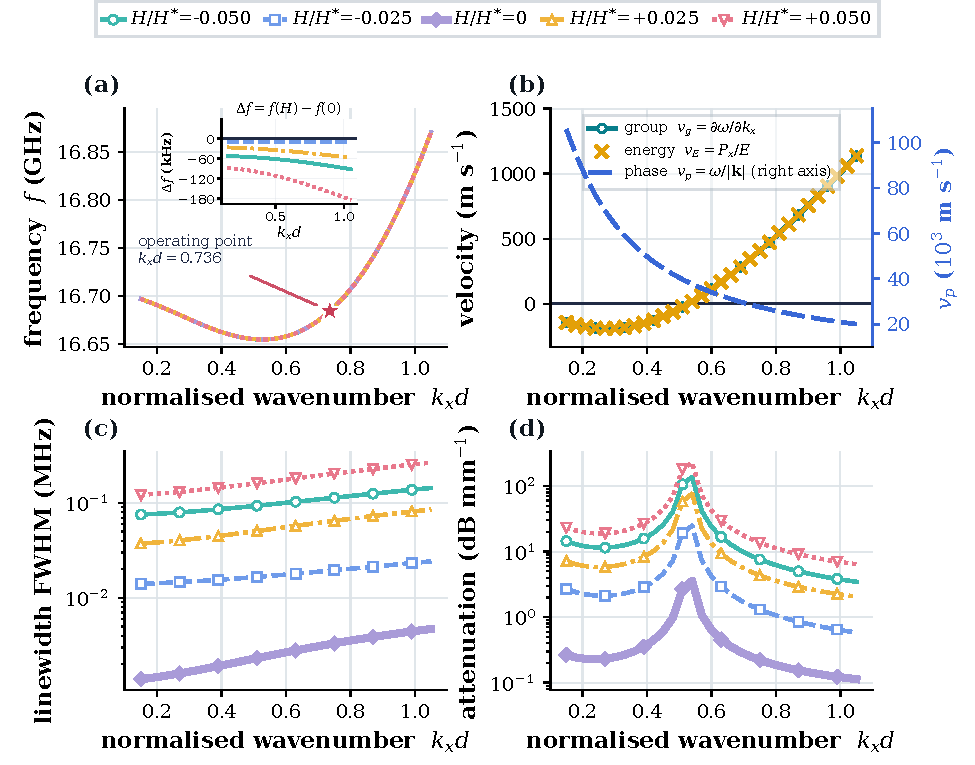
\includegraphics[width=0.95\textwidth]{figures/fig01_dispersion.pdf}
\caption{Guided branch at $k_yd=0.1298$, $d=\SI{200}{\nano\metre}$, $\ell=\SI{50}{\nano\metre}$. (a) Frequency against $k_xd$, with the inset showing $\Delta f=f(H)-f(0)$; the operating point $k_xd=0.736$ is marked. (b) Group, energy and phase speeds at $H=0$. (c) Linewidth and (d) attenuation, $4.343\times2|\Imag k_x|$ in dB mm$^{-1}$, for five coupling levels.}
\label{fig:fig01}
\end{figure}


Before the numbers are read, the part of \eqref{eq:enthalpy} exercised by the calculations should be stated.

Four sectors are active in each solve: the elastic, the strain-gradient, the
piezoelectric and the carrier sector.  The flexoelectric sector is active but
subdominant.  A single flexoelectric constant $f\equiv f_{3zz}=\SI{1}{\nano
\coulomb\per\metre}$ is retained.  It lies at the low end of the range
reported for ZnO \cite{hu2025computational,zhao2021effects} and is an assumed value, taken independently of the
crystal used for the elastic constants; it gives the dimensionless
coupling $f=2.56\times10^{-3}$ of \cref{tab:groups}.  The added
carrier--strain-gradient coupling is swept over
$|H|\le\SI{2.0e-23}{\joule\metre}=0.022\,H_{\text{bound}}$, i.e.\ over the
range allowed by \eqref{eq:schur}.

The flexoelectric term was tested directly, by repeating the two solved configurations with $f$ set to zero and to ten times
the retained value.  At the
operating point the backward
channel is $0.0192916$ with the retained $f$ and $0.0192938$ with $f=0$, a
change of \SI{-0.012}{\percent}; at $k_xd=0.55$ it is $0.551910$ and
$0.551976$, a change of \SI{-0.012}{\percent}.  At ten times the retained value the changes
are \SI{-1.16}{\percent} and \SI{-1.18}{\percent}, so the dependence is smooth
and quadratic in the coupling (a factor of 97 for a factor of ten), with no threshold.

Taken together, these numbers place the reported shares within one part in ten
thousand of the shares of the \emph{strain-gradient
piezoelectric-semiconductor} specialization with the added carrier coupling.
The flexoelectric term is present and contributes with the correct sign and
magnitude, and it does not drive the effect.  What the numbers support is a
slow-mode edge effect of the strain-gradient plate, modulated by the carrier
coupling, inside a flexoelectric-semiconductor formulation; they do not support
the attribution of the negative reflection to the flexoelectric mechanism
itself.

\subsection{Dependence on carrier density, thickness and frequency}
\label{sec:results_material}
\label{sec:results_geometry}
\label{sec:results_frequency}

\Cref{fig:fig02} sweeps the two material families.  Increasing the carrier
density from $1$ to $3\times10^{18}\,\si{\per\cubic\metre}$ raises the linewidth
(a) and the attenuation (b) by a factor of three each (the conduction loss is
linear in the density over this range) and lowers the frequency only
slightly.  Panel (c) is the most informative: the backward channel at the reference plane is plotted against
$k_xd$ for the five densities, and the five curves collapse onto one.  The
largest sampled value, $R_B\approx0.552$ ($0.5515$ to $0.5523$), is at $k_xd=0.55$ for all densities; this raster of $\Delta k_xd=0.05$ does not resolve the fold at $k_xd=0.527$, whose maximum is given in \cref{sec:results_peak}.  The
relative spread between the five curves is below \SI{0.2}{\percent} over the full range.  On this raster, and over this factor-of-three range, the carrier density thus sets the loss but not the partition of the scattered power (see \cref{sec:results_sens} for a wider range).

The mobility behaves in the same way (panel d): over the factor-of-three range
$0.00875$ to $0.02625\,\si{\square\metre\per\volt\per\second}$ the linewidth
changes by the same factor of three, while the backward share is unchanged to
the same $0.2$ percent.  The two sweeps agree row by row because both quantities enter the conduction
term through their product, while the density also enters the screening through
$Q^{2}=5.6\times10^{-3}$, which is small here; the two are therefore equivalent at this $Q$ and not interchangeable in
general (see \cref{sec:results_sens} for larger densities).  Both results are consistent with $Q=d/L_D=0.075<1$: the
plate is thinner than the Debye length, the carrier perturbation is not confined
to a surface layer, and the density enters the problem mainly through the
conduction loss.

Every row of this sweep satisfies the conservation bound \eqref{eq:admissible}; the curve in panel (c) extends to $k_xd=0.9$, falling below
$10^{-7}$ beyond $k_xd=0.8$ and reaching between $3\times10^{-12}$ and $1\times10^{-11}$ at the last sample.  This is the backward port ceasing to carry energy, not a numerical failure.  Rows at that end have $|\cos\theta_E|\to0$, and the flux
fraction is evaluated at each point so that the loss of resolution is visible.

\begin{figure}[htbp]
\centering
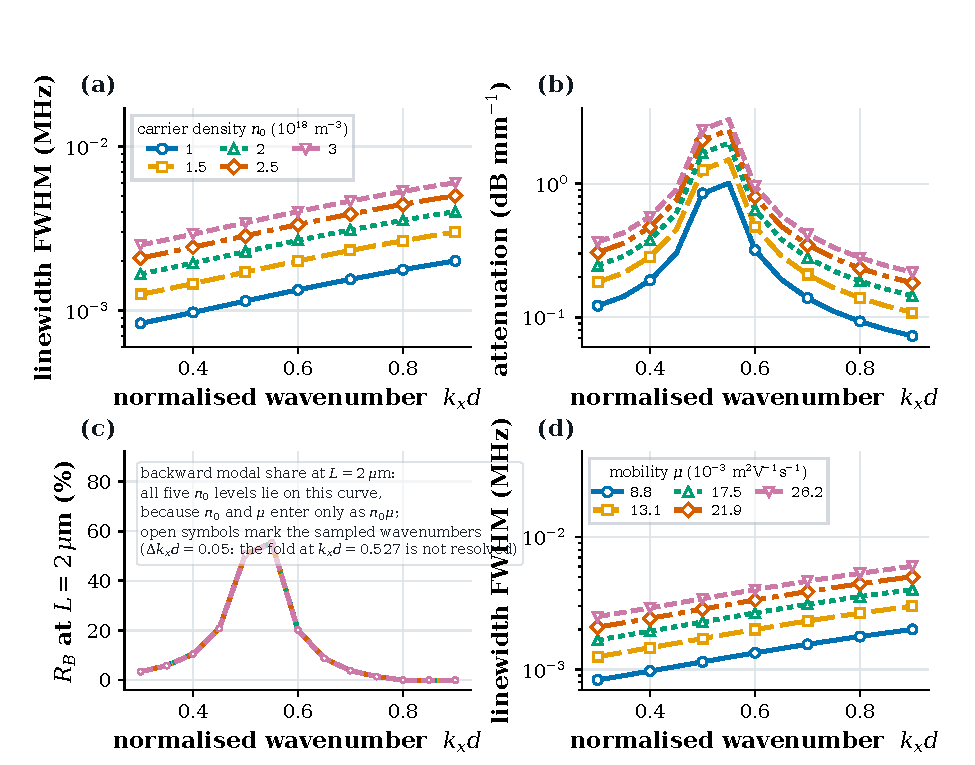
\includegraphics[width=0.95\textwidth]{figures/fig02_material.pdf}
\caption{Carrier density and mobility at $H=0$, $k_yd=0.1298$, sampled every $\Delta k_xd=0.05$. (a) Linewidth and (b) attenuation ($4.343\times2|\Imag k_x|$) for five $n_0$; (c) backward share at $L=\SI{2}{\micro\metre}$; (d) linewidth for five mobilities.}
\label{fig:fig02}
\end{figure}


\Cref{fig:fig03} separates the two geometric families, which scale differently
and must not be plotted on a common axis.  Plate thickness is the dominant
scale: across the family between \SI{120}{\nano\metre} and \SI{320}{\nano\metre}
the branch lies between \SI{10.5}{\giga\hertz} and \SI{30.4}{\giga\hertz}, and
the relative change is of order unity at all wavenumbers (panels a and c).  The gradient length shifts the same
branch by a smaller amount than the thickness (panels b and d): relative to
$\ell=\SI{50}{\nano\metre}$, a change to $\ell=\SI{90}{\nano\metre}$ shifts the
frequency by \SI{+2.0}{\percent} at $k_xd=0.145$ and by \SI{+10.2}{\percent} at
$k_xd=1.00$, while $\ell=\SI{35}{\nano\metre}$ shifts it by \SI{-1.9}{\percent}
and \SI{-4.9}{\percent} at the same two points.  The sign of the effect changes
with $\ell$ across the reference value, so the panel is plotted as a
relative change and not as an absolute frequency.

The distinction matters for the interpretation of the rest of the paper.  A
thickness change rescales the whole problem and is not a coupling effect; a
gradient-length change alters the relative weight of the hyperelastic and
flexoelectric terms at fixed geometry and so is the parameter that belongs with $H$ in a discussion of the added physics.

\begin{figure}[htbp]
\centering
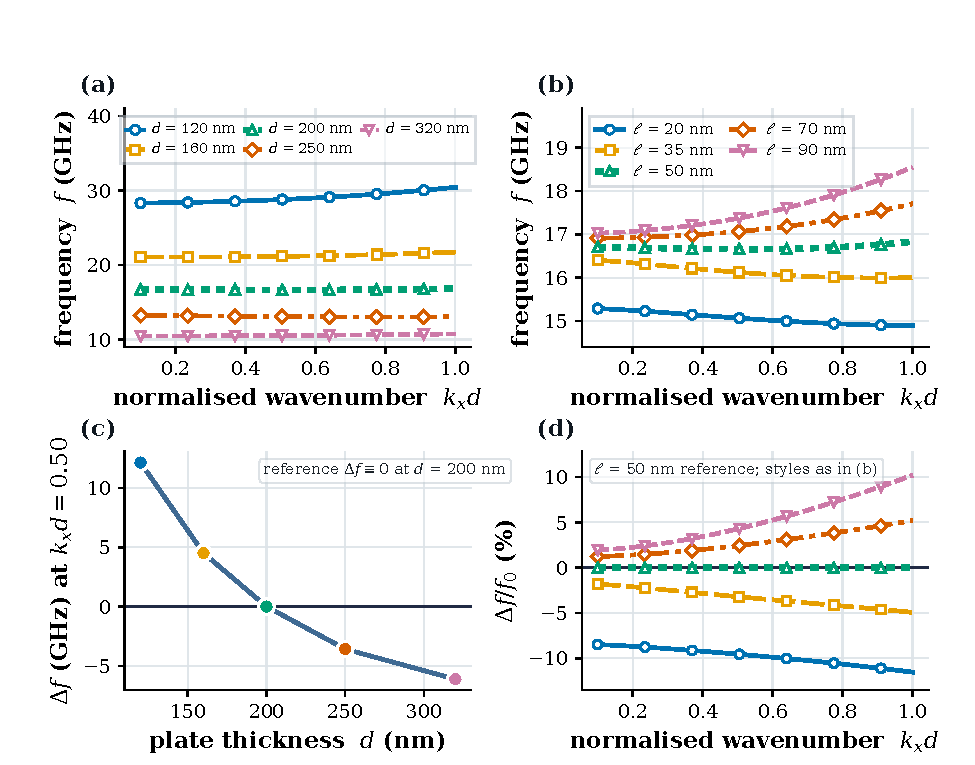
\includegraphics[width=0.95\textwidth]{figures/fig03_geometry.pdf}
\caption{Thickness and gradient length at $H=0$, $k_yd=0.1298$. (a) Dispersion for five thicknesses ($\ell=\SI{50}{\nano\metre}$); (b) dispersion for five gradient lengths ($d=\SI{200}{\nano\metre}$), each the operating-point branch followed from $\ell=\SI{50}{\nano\metre}$; (c) $\Delta f$ at $k_xd=0.50$ against thickness; (d) relative frequency change for five gradient lengths.}
\label{fig:fig03}
\end{figure}


\Cref{fig:fig04} sweeps the drive along the solved guided branch, not at a fixed frequency.  This matters away from the operating point, where
a fixed-frequency solve does not return the physical continuation of the branch
and the energy angle collapses towards $-90^{\circ}$; following the branch gives,
for each row, a resolved triple of frequency, wavenumber and share.  Two
rasters are used: a coarse one over the full window and, at $H=0$ only, a fine
one of spacing $\Delta k_xd=5\times10^{-4}$ across $0.520\le k_xd\le0.535$,
because the top of the response is three orders of magnitude narrower than any
raster that can be drawn on a single axis.  The number of rows is a property of
the grid.

The share along the branch is largest on its slow part.  It is $0.0341$
at $k_xd=0.30$ ($f=\SI{16.676}{\giga\hertz}$), rises to $0.9429$ at
$k_xd=0.52719$ ($f=\SI{16.6547}{\giga\hertz}$), and falls to $0.0142$ at
$k_xd=0.75$ ($f=\SI{16.688}{\giga\hertz}$) (panel a).  The response has a single peak over the entire window: the coarse raster finds no second local
extremum, and the top of the peak is located by a refined search.  Panel (b) shows the signed energy angle
changing by $17^{\circ}$ across the window and passing through its own extremum
next to the maximum of $R_B$, so the two are not independent readings.  Panel (c)
plots the same data against the ratio $k_{Bx}/k_{ix}$: all five coupling levels
collapse onto one master curve, and the conversion is largest where the backward
wavenumber approaches the incident one, reaching $k_{Bx}/k_{ix}=0.9960$ at the
maximum.  The backward port is a propagating mode on the
backward-slope part of the same branch, not an evanescent artifact, and the projection onto it
becomes decisive where the two wavenumbers approach each other.  Panel
(d) shows why they do: the branch passes through a zero-group-velocity point at
$k_xd\approx0.527$, where $|v_g|$ falls below \SI{1}{\metre\per\second} against
$-187$ and $+409\,\si{\metre\per\second}$ at the two ends of the window, and the
incident and backward wavenumbers close on one another there and open again
beyond it.

\begin{figure}[htbp]
\centering
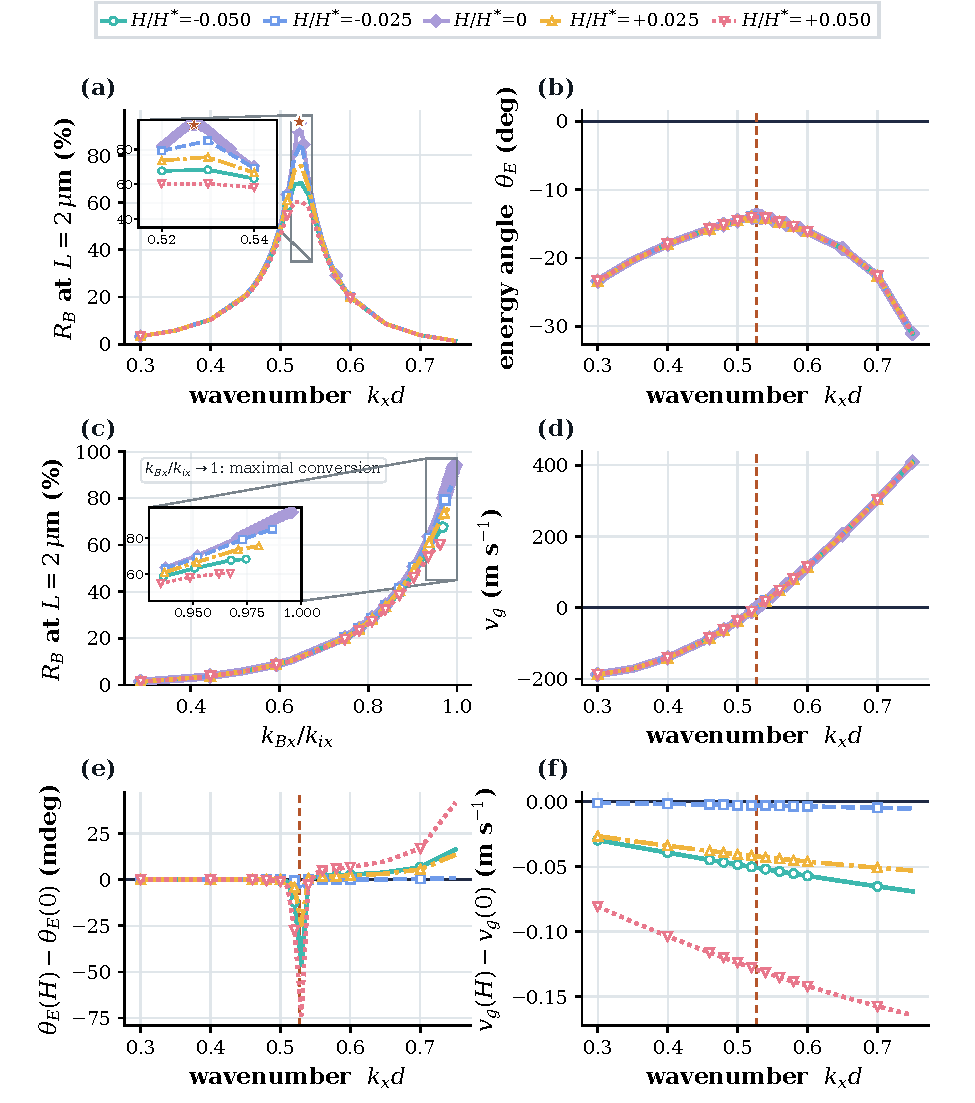
\includegraphics[width=0.95\textwidth]{figures/fig04_frequency.pdf}
\caption{Backward conversion along the branch at $k_yd=0.1298$, $L=\SI{2}{\micro\metre}$, with the frequency following the branch. (a) $R_B$ against $k_xd$, maximum marked by a star. (b) Energy angle. (c) $R_B$ against $k_{Bx}/k_{ix}$. (d) Group velocity. Insets magnify the region near the maximum; (e), (f) show the departure of (b) and (d) from $H=0$.}
\label{fig:fig04}
\end{figure}

In \cref{fig:fig04} the five coupling levels separate only near the maximum
(insets of panels a and c); the curves of panels (b) and (d) coincide on the
scale of the full response.  Panels (e) and (f) show that the energy angle
changes by at most $7\times10^{-2}$ degree, at the maximum, and the group
velocity by less than $0.2\,\si{\metre\per\second}$.  Every plotted row satisfies
the conservation bound \eqref{eq:admissible}.

\subsection{The branch maximum}
\label{sec:results_peak}
\label{sec:results_certification}

The maximum of \cref{fig:fig04} falls between two samples of the coarse raster, so it was solved again at six Galerkin degrees, each value being checked against the quadrature rule.  At degree $30$ the share is $0.019\,292$ at the operating point and $0.942\,872$ at the maximum.  Between degrees $14$ and $34$ the relative change of the maximum stays below $10^{-5}$ and that of the operating point is $2.5\times10^{-5}$, the successive changes decreasing monotonically; with the degree fixed at 22 and the rule taken from 64 to 256 nodes the maximum changes by less than $10^{-8}$.  The edge system is well conditioned (condition number at most $1.9\times10^{2}$, scaled edge residual below $3\times10^{-15}$), and the values are resolved projections: the energy angles are $-13.9^{\circ}$ and $-27.9^{\circ}$, so the measured $x$ flux is \SI{97.1}{\percent} and \SI{88.4}{\percent} of the total modal flux and neither value is an artifact of a near-grazing mode.

The quantity maximized is the one defined by \eqref{eq:RB}: the modal self-power of the identified backward outgoing mode at the reference plane, divided by the incident power at the same plane.  The other outgoing modes, the interference term and the dissipation are quoted separately and never folded into it.  A coarse raster of $\Delta k_xd=0.002$ over $0.465\le k_xd\le0.625$ (the whole window in which a backward port exists at this $k_y$) contains a single peak with its largest sample at $k_xd=0.527$, and a plateau raster of $10^{-4}$ and a refined raster of $10^{-5}$ place the maximum at $k_xd=0.52719$ with $R_B=0.9428718$.  The top is flat: every sampled wavenumber in $0.5267\le k_xd\le0.5276$ lies within \SI{0.01}{} percentage point of the maximum, so the reported location is the center of that top, determined to within $\pm0.0005$.  The incident wavenumber returned by the spatial problem is $k_{ix}d=0.52821$, \SI{0.19}{\percent} from the branch parameter, and no conclusion depends on the difference.  The result is a \emph{local maximum within the declared window}, not a global maximum over all $k_y$, thicknesses or material sets, none of which is searched here.

The maximum has a simple reading.  At the fold the group velocity vanishes ($+0.01\,\si{\metre\per\second}$ against $-187$ and $+409\,\si{\metre\per\second}$ at the ends of the solved window) and the backward and incident wavenumbers differ by \SI{0.4}{\percent}, so the two modes are nearly parallel and the edge conditions can be met with only a small admixture of the other outgoing modes; the projection onto the backward mode then takes almost all of the partition.  Panel (c) of \cref{fig:fig04} shows this: all coupling levels collapse onto one curve in $k_{Bx}/k_{ix}$, with the conversion maximal as the ratio approaches unity, and the conversion falls steeply on both flanks.  A grid of $\Delta k_xd=0.05$ would miss the maximum because the whole top of the response is $10^{-3}$ wide.  The same fold makes the incident flux fall by a factor of $131$ with respect to the operating point, so the partition is maximal where the transported power is minimal: that ninety-four percent of the energy is turned around would be true as a ratio and false as an energy budget, and only the ratio is claimed.  The outgoing propagating modes carry all of the incident power to within \SI{0.1}{\percent} (\cref{sec:results_channel}), so the plate is an almost perfect scatterer and the question is into which branch the power goes.  A measurement of the total reflectance would see essentially unity everywhere on the branch; the negative reflection requires modal resolution, by a wavenumber filter or a time-of-flight separation of the branches.

\subsection{Modal share and energy budget at the maximum}
\label{sec:results_artefact}
\label{sec:results_channel}

Three properties of the solution decide whether such a number can be read at
face value.

The incident flux at the maximum is small, a
factor $131$ below its value at the operating point, so the fraction could in
principle be a ratio of two nearly vanishing quantities.  It is not: the value
is reproduced to better than $10^{-5}$ across six Galerkin degrees, to
better than $10^{-8}$ across four quadrature rules, and to $2.3\times10^{-7}$ along three
different tracking paths that reach the same wavenumber from below, from above
and in a single step.  A ratio of two independently vanishing numbers would
scatter under all three.

The reference plane is moved from $0$ to $20$
thicknesses and the partition is rescaled by
$\exp[2(|\Imag k_{ix}|+|\Imag k_{Bx}|)(L-L_{\text{ref}})/d]$, which is the net
attenuation of the two partner modes travelling in opposite directions.  The
rescaled values agree to $2\times10^{-16}$, so the number is a property of the
edge and both attenuations are resolved and not assumed.  The transform is
applied identically to every result, and the edge-plane
fractions of the search, of the matched controls and of the coupling study
are reproduced by an independent re-evaluation to $10^{-10}$ relative or better; the plane at
which a share is quoted is hence a reporting choice and not a second
definition.  The backward port
is also unique: the second outgoing candidate lies $2.0|k_x|$ away, the
condition number of the normalized edge matrix is $1.4\times10^{2}$, and the
relative error bound of the projection is $\text{cond}\times\epsilon=4\times10^{-14}$.

The incident and backward eigenvectors
are nearly parallel, with overlap $0.999995$, and their wavenumbers are
separated by $1.45$ times the modal decay rate: close, but resolved.  The share also varies smoothly through the fold, taking the values $0.942\,777$, $0.942\,869$, $0.942\,872$, $0.942\,866$ and $0.942\,818$ at $k_xd=0.5267$, $0.5270$, $0.52719$, $0.5274$ and $0.5276$ at degree $22$, while the relative separation of the two wavenumbers stays within $0.2$ percent of its value at the maximum.  The
partition rebuilt from the amplitudes and modal powers alone reproduces the computed value to machine precision, which is the direct statement that no
eigenvector phase or scale enters the result.  What the near-coincidence does
change is interpretation, not accuracy: because the incident flux falls towards
the fold, the fraction is anti-correlated with it across the window, so a maximal share goes together with a minimal transported power.

The maximum is a modal share and not a reflectance.  At $k_xd=0.52719$ the
total outgoing propagating power is $1.00050$ of the incident power and the
interference correction at the reference plane is $+5.2\times10^{-4}$, so the
backward mode carries \SI{94.29}{\percent} of the incident power and
\SI{94.24}{\percent} of the outgoing propagating power.  At this fold the
interference term is sensitive at the level of $10^{-3}$ to the wavenumber at which the
frequency is fixed (it is $-8.0\times10^{-4}$ at the neighboring sample $k_xd=0.5275$, which has the same frequency to $10^{-8}$), whereas the modal share changes by $2\times10^{-5}$ relative.  The modal share is
\SI{94.29}{\percent}; the energy statement is that the propagating outgoing
modes carry the incident power to within \SI{0.1}{\percent}.  The two are different readings of the same
solution.

The maximum must also be read with its own amplitude in mind.  It lies on a zero-group-velocity fold, and a mode with vanishing group velocity carries
vanishing flux: the incident modal power per unit normalization falls from
$5.08\times10^{-3}$ at the operating point to $3.87\times10^{-5}$ at the
maximum, a factor $131$, while $|\Imag k_{ix}|d$ rises to $1.0\times10^{-3}$.
The fraction is the ratio of two small but resolved fluxes (well
defined, unchanged by the incident normalization, and stable to
$1\times10^{-5}$ under degree and quadrature refinement), but it is not a statement that a
large amount of energy is turned around.  Both readings are needed: the
partition is maximal at the fold and the transported power is minimal there.

The three configurations are compared term by term in
\cref{tab:configurations}.  Every entry is evaluated at degree 30, except the
attenuations, which are $2|\Imag k_x|/d$ formed from the same spatial roots and quoted in decibels of power ($4.343\times$).

\begin{table}[t]
\centering
\caption{The three reported configurations ($d=\SI{200}{\nano\metre}$, $\ell=\SI{50}{\nano\metre}$, $H=0$, $k_yd=0.1298$, $L=10d$). $R_B$ is a modal share, not a reflectance.}
\label{tab:configurations}
\scriptsize
\begin{tabular}{@{}lccc@{}}
\toprule
Quantity & Operating point & Maximum & $k_xd=0.55$ \\
\midrule
frequency & $\SI{16.684}{\giga\hertz}$ & $\SI{16.6547}{\giga\hertz}$ & $\SI{16.6550}{\giga\hertz}$ \\
longitudinal wavenumber $k_xd$ & 0.7362 & 0.52719 & 0.5500 \\
incident wavenumber $\Real k_{ix}d$ & 0.7362 & 0.5282 & 0.5500 \\
group velocity $v_g$ & $\SI{379}{\metre\per\second}$ & $\SI{0.01}{\metre\per\second}$ & $\SI{34}{\metre\per\second}$ \\
incident attenuation, $4.343\times2|\Imag k_{ix}|$ & \SI{0.235}{\deci\bel\per\milli\metre} & \SIrange{43.5}{44.5}{\deci\bel\per\milli\metre} & \SI{2.01}{\deci\bel\per\milli\metre} \\
backward attenuation, $4.343\times2|\Imag k_{Bx}|$ & \SI{0.227}{\deci\bel\per\milli\metre} & \SIrange{43.5}{44.5}{\deci\bel\per\milli\metre} & \SI{1.96}{\deci\bel\per\milli\metre} \\
backward share $R_B$ & $0.0192916$ & $0.9428718$ & $0.5519095$ \\
modal share at the edge plane & $0.0193$ & $0.9824$ & $0.5529$ \\
energy angle $\theta_E$ & $-27.90^{\circ}$ & $-13.85^{\circ}$ & $-14.45^{\circ}$ \\
total outgoing propagating power & $0.99980$ & $1.00050$ & $0.99878$ \\
interference $P_{\text{cross}}/P_{\text{inc}}$ & $-4.6\times10^{-6}$ & $+5.2\times10^{-4}$ & $-1.03\times10^{-3}$ \\
dissipation $P_{\text{diss}}/P_{\text{inc}}$ & $1.99\times10^{-4}$ & $2.78\times10^{-5}$ & $1.93\times10^{-4}$ \\
edge-system condition number & $\le 2\times10^{2}$ & $\le 2\times10^{2}$ & $\le 2\times10^{2}$ \\
scaled edge residual & $\le3\times10^{-15}$ & $\le3\times10^{-15}$ & $\le3\times10^{-15}$ \\
\bottomrule
\end{tabular}
\end{table}


\Cref{fig:fig05} closes the energy identity \eqref{eq:energy_identity} at the
reference plane.  At $H=0$ the incident power normalized to unity is partitioned
as follows: the identified backward channel carries $1.9292\times10^{-2}$, the
remaining propagating outgoing modes carry $0.980505$, dissipation removes
$1.989\times10^{-4}$, and the interference term is $-4.6\times10^{-6}$.  The
first two sum to $0.999796$, the total outgoing propagating power; adding the
dissipation leaves $5\times10^{-6}$ of the incident power, which is the magnitude of the interference term to the six digits quoted.  The
interference term is defined as the remainder of the identity, so the sum closes
by construction; the independent check is the balance of the flux at the
reference plane against the edge flux and the conduction loss, which closes to
better than $10^{-11}$ relative at each Galerkin degree from 14 to 34, five
orders of magnitude below the $10^{-6}$ threshold plotted in panel (c).  At the maximum
the backward channel carries $0.942872$ and the remaining propagating modes
$5.76\times10^{-2}$, which together account for $1.00050$ of the incident
power; dissipation removes $2.78\times10^{-5}$ and the interference term is
$+5.2\times10^{-4}$.  The same power balance closes there to
$6\times10^{-14}$.

The evanescent spectrum does not belong to the transported budget.  At the
reference plane the entire evanescent content has decayed by a factor
$\exp(-2|{\Imag k_x}|L)$ with $|{\Imag k_x}|L\gtrsim10$, which leaves
$4.8\times10^{-28}$ of the incident power.  Reactive accounting is meaningful
only at the edge plane, where it is $4.4\times10^{-6}$, and even there it
is not transported energy.  For the same reason $P_{\text{cross}}$ is an
interference correction and not a channel, and the evanescent members of
$\{P_j\}$ are reactive; the complete statement is the partition above, with the
interference term quoted explicitly.

Panels (b) and (d) sweep the coupling at the \emph{fixed} operating frequency
$\omega=\omega_0$, so the incident wavenumber drifts with $H$ along the branch
instead of the frequency doing so.  That is the response of the plate driven at
one frequency; the branch-consistent comparison is the relevant one.  At
fixed frequency the backward channel changes from $1.9051\times10^{-2}$ at
$H/H^{*}=-0.05$ to $1.8876\times10^{-2}$ at $H/H^{*}=+0.05$, a variation of
\SI{0.92}{\percent}; dissipation rises from $6.9\times10^{-3}$ to
$1.2\times10^{-2}$; the other propagating modes carry the balance.  Panel (d)
gives the same information as a relative change against the uncoupled baseline:
the largest deviation is \SI{-2.15}{\percent} at $H/H^{*}=+0.05$.  When instead
$k_x$ is held fixed and the frequency follows the branch (the branch-consistent comparison), the deviation at the same tabulated extreme is
\SI{-1.21}{\percent}: part of the fixed-frequency variation is the dispersion
shift of $H$, which reaches $6.3\times10^{-5}$ in $\omega$.

\begin{figure}[htbp]
\centering
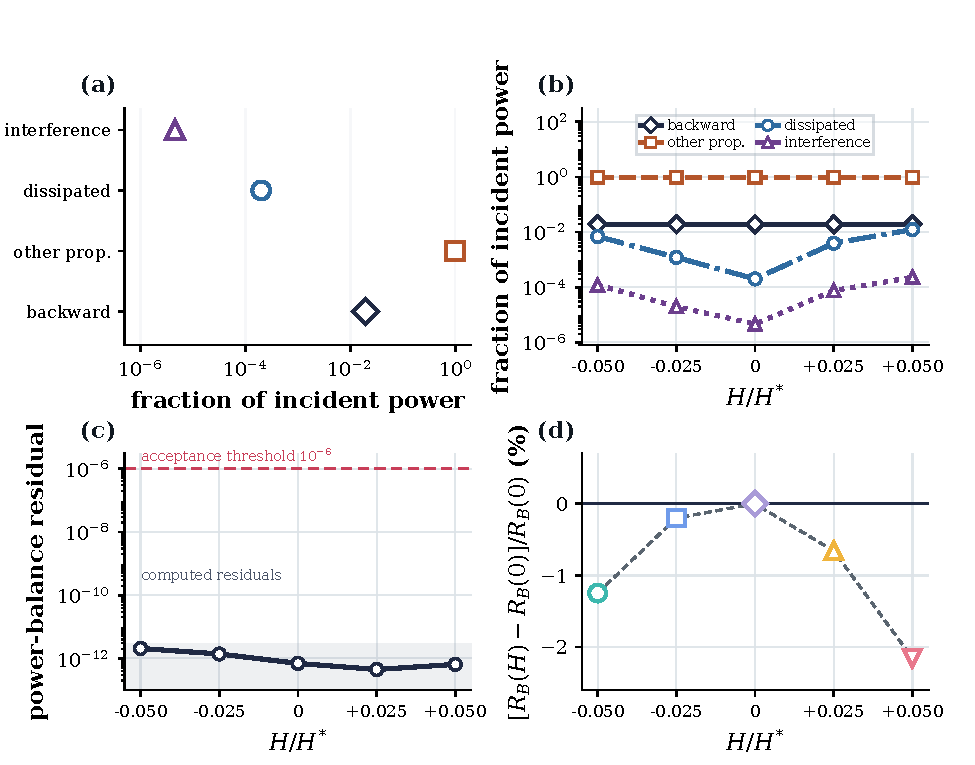
\includegraphics[width=0.95\textwidth]{figures/fig05_channel.pdf}
\caption{Energy budget at the operating point and the reference plane $x=-10\,d$; the interference term is shown as a magnitude. (a) Partition at $H=0$. (b) The same fractions against $H/H^{*}$ at fixed frequency. (c) Power-balance residual. (d) Relative change of the backward channel.}
\label{fig:fig05}
\end{figure}

\subsection{The backward channel}
\label{sec:results_mechanism}
\label{sec:results_attenuation}

The partition quoted above was computed at $H=0$, with the
carrier--strain-gradient coupling switched off, and the contribution of that
coupling is isolated by matched controls: each ingredient except the named one
is held fixed (same $k_x$, same $k_y$, same $n_0$, same $\ell$, same reference
plane, same unit incident self-power), and the frequency follows the branch,
because switching an ingredient off changes the dispersion and solutions taken at
different frequencies of a different branch would not be comparable.
\Cref{tab:controls} lists the outcome.

\begin{table}[t]
\centering
\caption{Matched controls. The frequency follows the branch. Entries marked ``sp'' are specular self-powers, not backward conversion.}
\label{tab:controls}
\footnotesize
\begin{tabularx}{\textwidth}{@{}>{\raggedright\arraybackslash}Xcccccc@{}}
\toprule
 & \multicolumn{2}{c}{Operating point ($k_xd=0.736$)}
 & \multicolumn{2}{c}{Maximum ($k_xd=0.52719$)}
 & \multicolumn{2}{c}{$k_xd=0.550$} \\
\cmidrule(lr){2-3}\cmidrule(lr){4-5}\cmidrule(lr){6-7}
Configuration & freq.\ (GHz) & $R_B$ & freq.\ (GHz) & $R_B$ & freq.\ (GHz) & $R_B$ \\
\midrule
full ($f_0$, $H/H^{*}=+0.05$) & 16.6840 & 0.019\,058 & 16.6546 & 0.602\,292 & 16.6549 & 0.495\,776 \\
$f=f_0$, $H=0$                & 16.6841 & 0.019\,292 & 16.6547 & 0.942\,872 & 16.6550 & 0.551\,910 \\
$f=0$, $H/H^{*}=+0.05$        & 16.6840 & 0.019\,060 & 16.6546 & 0.602\,290 & 16.6549 & 0.495\,822 \\
$f=0$, $H=0$                  & 16.6841 & 0.019\,294 & 16.6547 & 0.942\,878 & 16.6550 & 0.551\,976 \\
$\ell=0$, $f=0$, $H=0$        & 16.2077 & 0.075\,961$^{\mathrm{sp}}$
                              & 15.9717 & 0.133\,278$^{\mathrm{sp}}$
                              & 15.9943 & 0.124\,109$^{\mathrm{sp}}$ \\
\bottomrule
\end{tabularx}
\end{table}

Three statements follow.

First, the effect is already present with $H=0$: the same branch converts
\SI{1.93}{\percent} at the operating point and \SI{94.29}{\percent} at the
maximum.  The strain-gradient piezoelectric-semiconductor model already contains the partition, and the coupling can only modify it.

Second, the size of the modification depends strongly on where the branch is
sampled, and it is quantified.  Turning $H$ on at the tabulated extreme
$|H|=0.05H^{*}$ \emph{reduces} the partition by \SI{1.21}{\percent} at the
operating point, by \SI{10.17}{\percent} at $k_xd=0.55$ and by
\SI{36.1}{\percent} at the maximum.  The flexoelectric coefficient is
neutral by comparison: at $f_0=\SI{1}{\nano\coulomb\per\metre}$ it moves the
partition by \SI{-0.012}{\percent} at the operating point, by
\SI{-0.012}{\percent} at $k_xd=0.55$ and by \SI{0.0004}{\percent} at the
maximum.  The mechanism of the reduction is
attenuation of both partner modes, whose decay rate rises from
$1.0\times10^{-3}$ to $8.5\times10^{-3}$ per unit thickness at the maximum, so a
larger part of the conversion is lost between the edge and the reference plane:
referred to the edge plane, where both effects are evaluated at the same place,
the reduction is \SI{13.8}{\percent}, whereas it is \SI{36.1}{\percent} at the reference plane, and the
remaining 22.3 percentage points are propagation loss.  At $k_xd=0.55$ the same
comparison gives \SI{1.65}{\percent} at the edge plane, against \SI{-10.17}{\percent} at the reference plane: there the
coupling slightly \emph{raises} the edge-plane share, and the whole of the
reference-plane reduction is propagation loss.  The
branch-consistent sweep is monotone in $|H|$: at the maximum
$R_B=0.9429$, $0.7564$, $0.6023$ for $H/H^{*}=0$, $+0.025$, $+0.05$ and
$0.8541$, $0.6827$ for $-0.025$, $-0.05$.  When the extremum is re-searched
afresh at each coupling level it moves to $k_xd=0.5222$, $0.5292$, $0.5272$,
$0.5279$, $0.5240$ for $H/H^{*}=+0.05$, $+0.025$, $0$, $-0.025$, $-0.05$, and
the largest attainable share falls to $0.6034$ and $0.6832$ at the two extremes,
so the coupling lowers the upper bound as well as shifting the location, and the
shift is not monotone in the sign of $H$.

Third, the gradient length fixes the frequency and the wavenumber of the fold;
it does not create the backward interval.  At the control frequencies of the last
row of \cref{tab:controls}, which lie on a different classical branch from the continuation followed below, the classical plate ($\ell=0$) has no outgoing mode with
positive axial wavenumber and negative axial power: the only negative-power
outgoing mode is the specular reflection, whose wavenumber equals $-k_{x,\text{inc}}$; those entries therefore carry the superscript ``sp''.
Following the operating-point mode to $\ell=0$ at fixed $k_y$, however, shows that
the classical plate has a backward interval of its own.  Along that path the frequency at $k_x=K_0$ falls from \SI{16.684}{\giga\hertz} to \SI{13.687}{\giga\hertz}, the fold moves from $k_xd=0.527$ at $\lambda=0.25$ to $k_xd=0.824$ at $\lambda=0$ (through $1.084$ at $\lambda=0.10$), and the group velocity is negative below the fold for every value of $\lambda$ sampled.


The branch is tracked by modal overlap (at least $0.998$ between neighboring steps), the group velocity is $\dd\Omega/\dd K$ by finite differences with $\Delta K=0.01$, and the results agree to four digits between Galerkin degrees 18 and 24.


The edge problem was solved for the classical plate ($\lambda=0$, no flexoelectricity, no
coupling) at the fold of the tracked branch: at $k_xd=0.824$ and
$\SI{13.6855}{\giga\hertz}$ the backward mode carries $0.83620$ of the incident power at the
reference plane, and at $k_xd=0.95$ ($\SI{13.6891}{\giga\hertz}$) it carries $0.95904$.  The spectral
expansion at degrees $18$ and $26$ and the independent $C^{1}$ finite-element plate with $24$
elements agree to $9\times10^{-9}$ (first point) and $4\times10^{-8}$ (second point), the power
balance closes to $3\times10^{-11}$ or better, and the scaled edge residual is below
$3\times10^{-15}$.  The large backward share is present in the classical plate before any
strain-gradient length is introduced.

Taken together, the results read as follows.  The negative
reflection is a property of the backward guided branch: on it the energy flux
travels opposite to the phase, the free edge converts into it, and, at $\lambda=0.25$, the conversion
is largest where the branch group velocity vanishes; the gradient length
determines where that fold lies.  The carrier dynamics determine the attenuation
of both branches and so the observed value at a finite reference plane.
The added carrier--strain-gradient coupling acts through that attenuation: it
leaves the partition almost untouched where the branch is fast, and removes a
third of it at the slow point, because there the conversion is large and the
added decay has the whole distance to the reference plane to act.  It modifies
the picture; it does not create it.


\Cref{fig:fig06} follows the two channels away from the edge.  The backward
coefficient decays with the observation distance $L$ (panel a) as
$\exp(-\alpha_B L)$ with $\alpha_B=2|\Imag k_{Bx}|$, and the incident power
arriving at the edge obeys a survival factor normalized to its edge value, which cannot exceed unity (panel b); the minimum over the solved range, reached at $H/H^{*}=+0.05$, is
$0.0356$ at $L=\SI{1000}{\micro\metre}$, one millimeter from the edge.

Panels (c) and (d) give the attenuation length and the loss coefficient against
the coupling.  Both are obtained from the complex spatial roots,
$\alpha=2|\Imag k_x|$, and neither is derived from a real square root.  The
attenuation length is largest at $H=0$ ($\approx\SI{18}{\milli\metre}$) and
falls by more than an order of magnitude at either extreme of the coupling
range, to \SI{0.54}{\milli\metre} at $H/H^{*}=-0.05$ and to
\SI{0.30}{\milli\metre} at $+0.05$, and the loss
coefficient follows the same pattern with a minimum of
\SI{0.23}{\deci\bel\per\milli\metre} at $H=0$ and a maximum of
\SI{14.5}{\deci\bel\per\milli\metre} at $H/H^{*}=+0.05$; the corresponding
attenuation length falls from \SI{18.5}{\milli\metre} to
\SI{0.30}{\milli\metre}, a factor of sixty-two.  The incident and backward
channels share the same attenuation only at $H=0$ (0.235 and \SI{0.227}{\deci\bel\per\milli\metre}); away from it
they separate strongly, reaching 8.08 and
\SI{11.5}{\deci\bel\per\milli\metre} at $H/H^{*}=-0.05$.  The coupling thus controls the loss of the plate much
more strongly than it controls the partition of the scattered power, which is
the opposite of what one might expect from the magnitude of the term
\eqref{eq:added_coupling} alone.

\begin{figure}[htbp]
\centering
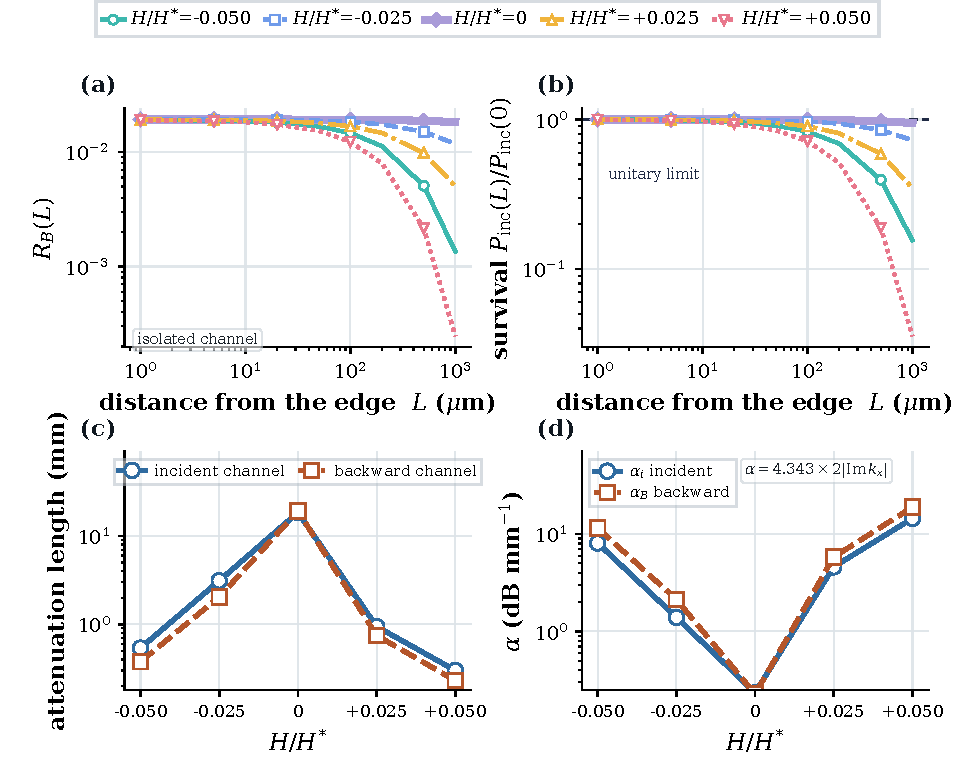
\includegraphics[width=0.95\textwidth]{figures/fig06_attenuation.pdf}
\caption{Distance, survival and attenuation at the operating point. (a) Backward channel against distance from the edge; (b) incident-power survival factor, normalized to its edge value; (c) attenuation length ($1/\alpha$ with $\alpha=2|\Imag k_x|$) and (d) loss coefficient in dB mm$^{-1}$ ($4.343\,\alpha$) against $H/H^{*}$.}
\label{fig:fig06}
\end{figure}

\subsection{Coupling and the through-thickness flux}
\label{sec:results_coupling}
\label{sec:results_boundary}

\Cref{fig:fig07} resolves the two-parameter dependence.  Over the solved box
$0.05\le k_yd\le0.20$ and $-0.05\le H/H^{*}\le0.05$, the backward channel ranges
from $0.01546$ to $0.02180$.  Panel (a) shows that the transverse wavenumber
alone accounts for almost all of that range: the five coupling curves are
displaced but their common slope is set by $k_y$.  Panels (c) and (d) quantify
the displacement: against $H/H^{*}$ at fixed operating frequency the relative
change is at most \SI{2.48}{\percent}, and against $k_y$ it is a slow drift that
never exceeds the same bound.  The ratio of the two sensitivities is the
quantitative statement of this paper about the added coupling: $k_y$ changes the
backward channel by a factor of $1.41$ across the box, while $H$ changes it by
at most \SI{2.5}{\percent} at fixed frequency and by \SI{1.21}{\percent} in the
branch-consistent comparison.  The coupling is a
perturbation of the partition and not its organizing parameter.  The comparison
must be made at fixed $k_x$, because it is the branch and not the coupling that
sets the partition; the two sensitivities do meet, however, at the branch
maximum, where the branch-consistent coupling effect grows to
\SI{36.1}{\percent}.  The $k_y$ sweep of \cref{fig:fig07} was solved at the operating point only.

Panel (b) draws the computed $5\times19$ grid cell by cell, with no
interpolation beyond the computational box and no smoothing between the five
coupling levels.  Every row of the grid satisfies \eqref{eq:admissible}.

\begin{figure}[htbp]
\centering
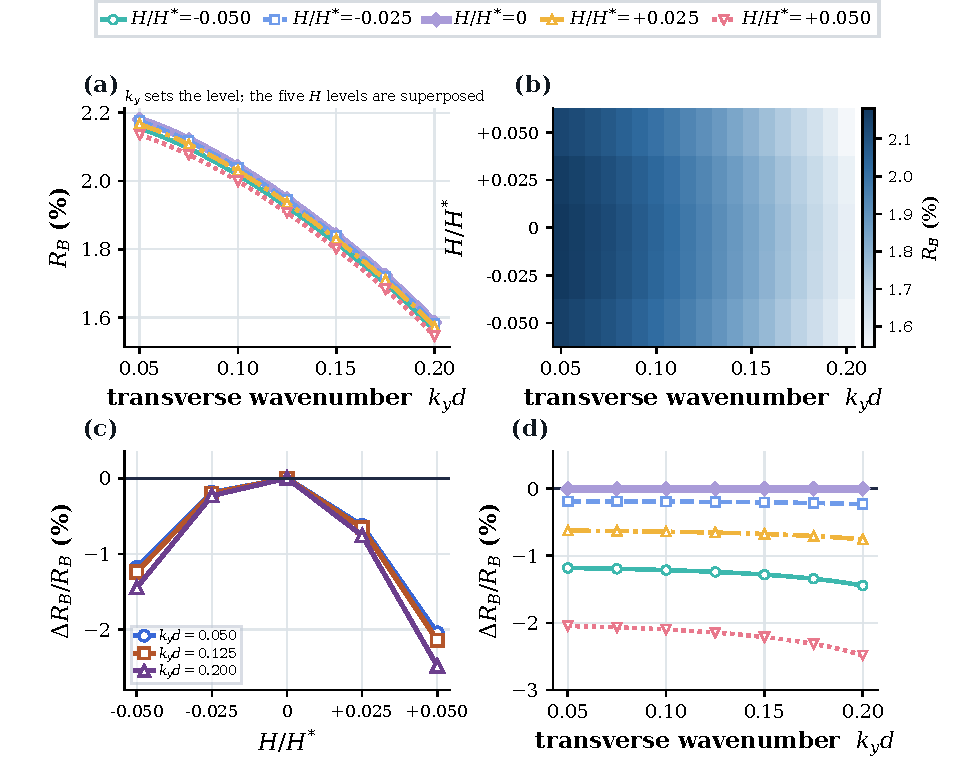
\includegraphics[width=0.95\textwidth]{figures/fig07_coupling.pdf}
\caption{Coupling sensitivity at the operating frequency and wavenumber $k_xd=0.7362$ (the operating point has $k_yd=0.1298$). (a) $R_B$ against $k_yd$ for five $H/H^{*}$; (b) measured $R_B(k_yd,H)$ grid; (c) relative change against $H/H^{*}$ for three $k_yd$; (d) relative change against $k_yd$.}
\label{fig:fig07}
\end{figure}


\Cref{fig:fig08} examines how the backward flux is distributed through the
thickness.  The plotted quantity is the $x$ component of the backward Poynting
flux, normalized by the incident flux, as a function of $z/d$; it is an
evaluated field, not an interpolated surface.

The distribution is a signature of the mode and not of the edge.  The $x$ component
changes sign inside the plate: it is positive near both free surfaces and
negative in the core, reaching $-0.0306$ and $+0.0264$ in units of the thickness-integrated incident flux, while its thickness integral remains negative.  The net backward power is carried by a mode whose local flux direction alternates across the
thickness, which follows from the strain-gradient plate mode itself.  The $z$ component behaves differently: it is largest at the free
surfaces and does not vanish there, so the surfaces carry a transverse flux even
though both traction and double traction vanish on them.  This is the
configuration in which the reactive near field must be retained at the edge
plane, and it explains why the energy budget separates the reactive content from
the transported content instead of adding them.

Panel (c) gives the running thickness integral normalized to its own total, so
the curve rises from zero to one across the plate for each coupling level and
the five curves are indistinguishable.  Panel (d) compares the shape of the
backward and incident $x$ fluxes at $H=0$, both normalized by their own maxima;
both profiles are symmetric about the mid-plane, the incident flux lies mostly near the two faces
(\SI{55}{\percent} of $\int|P_x|\,\dd z$ within $0.1\,d$ of them) and the backward flux does not
(\SI{9}{\percent}).

\begin{figure}[htbp]
\centering
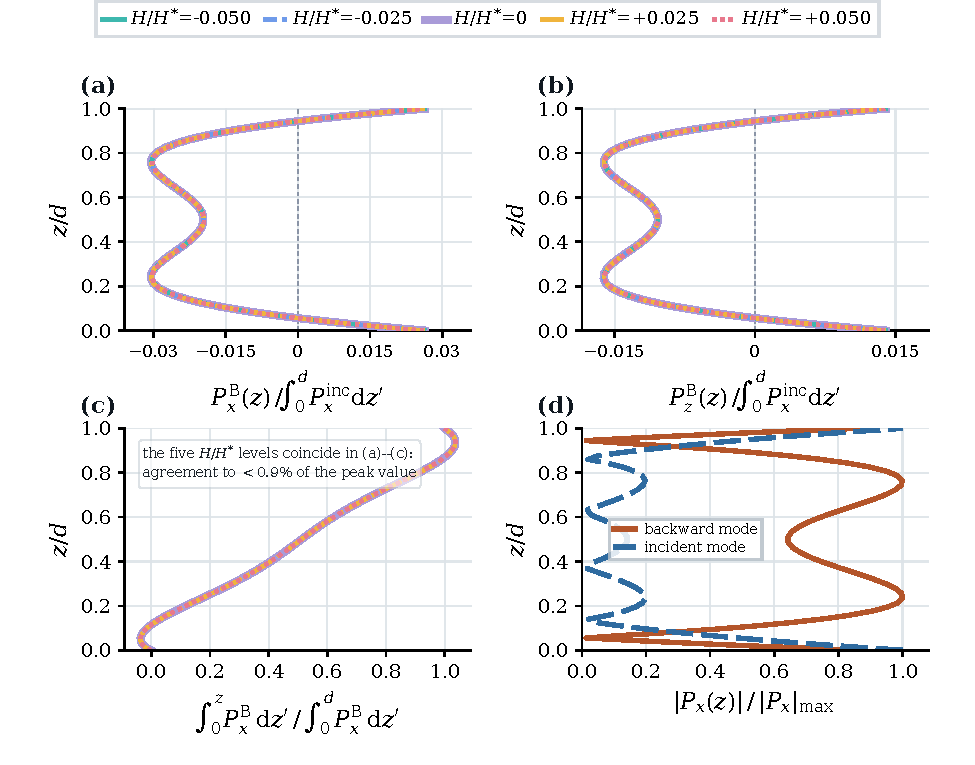
\includegraphics[width=0.95\textwidth]{figures/fig08_boundary.pdf}
\caption{Through-thickness backward flux at the operating point and the reference plane, in units of the thickness-integrated incident flux $\int_0^dP_x^{\mathrm{inc}}\,\dd z$. (a) $P_x^{\mathrm{B}}(z)$ and (b) $P_z^{\mathrm{B}}(z)$ for five $H/H^{*}$; (c) running integral of $P_x^{\mathrm{B}}$; (d) backward and incident $x$ fluxes at $H=0$.}
\label{fig:fig08}
\end{figure}

The coincidence of the five profiles in \cref{fig:fig08}(a)--(c) follows
from the assembly and not from a plotting choice, and it can be quantified.  The coupling enters through the two off-diagonal blocks that connect
the out-of-plane displacement to the carrier, whose entries are
\begin{equation}
\label{eq:H_entry}
\bigl(\mathsf A_{u\mu}\bigr)_{ij}
=h\int_{-1/2}^{1/2}b_i''(s)\,b_j(s)\,\dd s ,
\end{equation}
because $\widetilde\mu$ contains $-h\,\partial_s^{2}u_3$ and \eqref{eq:mu} is
the relation that conveys the coupling; written in the coordinate $\zeta=2s$ of
the field equations the same term acquires a factor four, $4\partial_\zeta^{2}$,
and the measure $\dd s=\dd\zeta/2$ is what keeps \eqref{eq:H_entry} free of it.
Since $b_i''$ has degree $i-2$ and $b_j$ has degree $j$, the matrix of
\eqref{eq:H_entry} vanishes unless $j\le i-2$: it is lower triangular, not upper triangular, and its row norms
$0,\,0,\,26.83,\,91.65,\,222.89,\,450.87,\,809.44$ at degree six grow with the
mode number as the second derivative does, the largest single entry being
$580.5$ in the last row.  With $h=1.06\times10^{-2}$
the largest entry of the assembled block is $6.13$, which is $10.5\%$ of the
inertia scale $\omega^{2}=58.3$ that sets the through-thickness balance of the
lowest rows, and four and a half orders of magnitude below the largest diagonal
entry of the same rows, $2.16\times10^{5}$.  That is a statement about the size of the
coupling, not about a mode: the operator is row-equilibrated before the
eigenvalue problem is formed, so no entry ratio is a frequency.  The size of these entries sets the scale of the coupling in the
assembled operator but is not used to derive the profile differences.  Those are
read from \cref{fig:fig08}(a)--(c): the flux profiles of the five levels differ by
less than \SI{0.9}{\percent} of the peak value, while the partition at the same
coupling changes by \SI{1.21}{\percent} at the operating point.

The same reading applies to the density sweep, where five carrier densities
collapse onto one curve.  The density enters the carrier sector only through the
screening group $Q^{2}=d^{2}q^{2}n_0/(\kappa_{33}k_BT)$, which multiplies the
single potential block $\mathsf A_{\varphi\mu}$, and through the mobility in
$\alpha_{\mathrm d}=\mu_ek_BT/(q\,d\,c_s)$; in the response the two appear as the
conductivity $n_0\mu_e$, so at fixed $n_0\mu_e$ the partition is unchanged and
the collapse reflects that product and not either parameter separately.

The ordering of these sensitivities is a property of the coupling and the operating point together: $k_y$ changes the backward channel by a factor of $1.41$ across the solved box while $H$ moves it by \SI{1.21}{\percent} at the operating point, but at the maximum the coupling moves the partition by \SI{36.1}{\percent}, and the $k_y$ sweep was not repeated there.  Any statement about the added coupling must therefore be made at fixed $k_y$, and an experimental attempt to see it must control the transverse wavenumber much better than the doping or the mobility.

\subsection{Validation and the near field}
\label{sec:results_validation}
\label{sec:results_field}

\Cref{fig:fig09} documents the numerical behavior of the edge solve.  Panels
(a) and (b) show the relative error of the backward channel and of the backward
wavenumber against the degree-33 reference: the channel error falls from
$2.6\times10^{-5}$ at $n=14$ to $1.6\times10^{-6}$ at $n=26$, while the wavenumber error remains at the $10^{-12}$ round-off floor over the full range, so the channel
error is still decreasing at the highest degree shown.  Panel (c)
shows the scaled edge residual and the relative energy-balance error for each degree: the residual is $3\times10^{-15}$, six to seven orders below the
$10^{-8}$ tolerance drawn in the panel, and the energy-balance error lies between $2\times10^{-13}$ and $4\times10^{-12}$, one to three orders below the
$10^{-10}$ line.  Both are round-off in a relative measure, and the panel
shows that neither drifts with the degree.  Panel (d) compares the temporal and spatial routes for the same
dispersion relation across the box; they agree to $2\times10^{-5}$.

The last panel is a check on the implementation, not a physical validation.  The
two routes discretize the same variational statement and differ only in which
variable is used as the eigenvalue; agreement to $2\times10^{-5}$ shows that the
assembly, the boundary conditions and the elimination of the potential are
implemented consistently.

The classical part of the edge solver was compared with the published
free-edge calculation of G\'erardin et al.\ \cite{gerardin2016negative}.  The
ZnO constants were replaced by those of their Duralumin plate ($\rho=\SI{2790}{\kilo\gram\per\cubic\metre}$,
$c_L=\SI{6398}{\metre\per\second}$, $c_T=\SI{3122}{\metre\per\second}$), with no piezoelectricity,
strain gradient or carrier coupling, and the incident $S_1$ mode was taken at normal incidence
($k_y=10^{-7}$ in the units of the solver).  The backward branch appears at
$f\times(2h)=\SI{2.8727}{\mega\hertz\milli\metre}$, against $2.87$ in \cite{gerardin2016negative}.  The
modal share $R_B=|r_{S_1|S_{2b}}|^2$ is $0.9988$ at
\SI{2e-6}{\mega\hertz\milli\metre} above that frequency, which is the
perfect conversion of \cite{gerardin2016negative}, and then falls to $0.797$, $0.500$ and
$0.288$ at $2.90$, $3.00$ and \SI{3.10}{\mega\hertz\milli\metre}, that is $|r|=0.893$, $0.707$ and $0.537$.
Read from their Fig.~2(b) by eye, the corresponding values are about $0.9$, $0.7$ and $0.55$, so the agreement is
within the reading accuracy of the figure; no tabulated values are available for a closer comparison.  Degrees 18 and 26 differ by
less than $10^{-9}$ in $R_B$, the power balance closes to $4\times10^{-11}$ and the edge residual is below $10^{-14}$.  This benchmark covers the classical elastic edge problem only; it does not test the
piezoelectric, strain-gradient or carrier terms.  The independent checks are the strong-form
integrations and the $C^1$ finite-element plate, neither of which shares the spectral matrices
with the production path.

\begin{figure}[htbp]
\centering
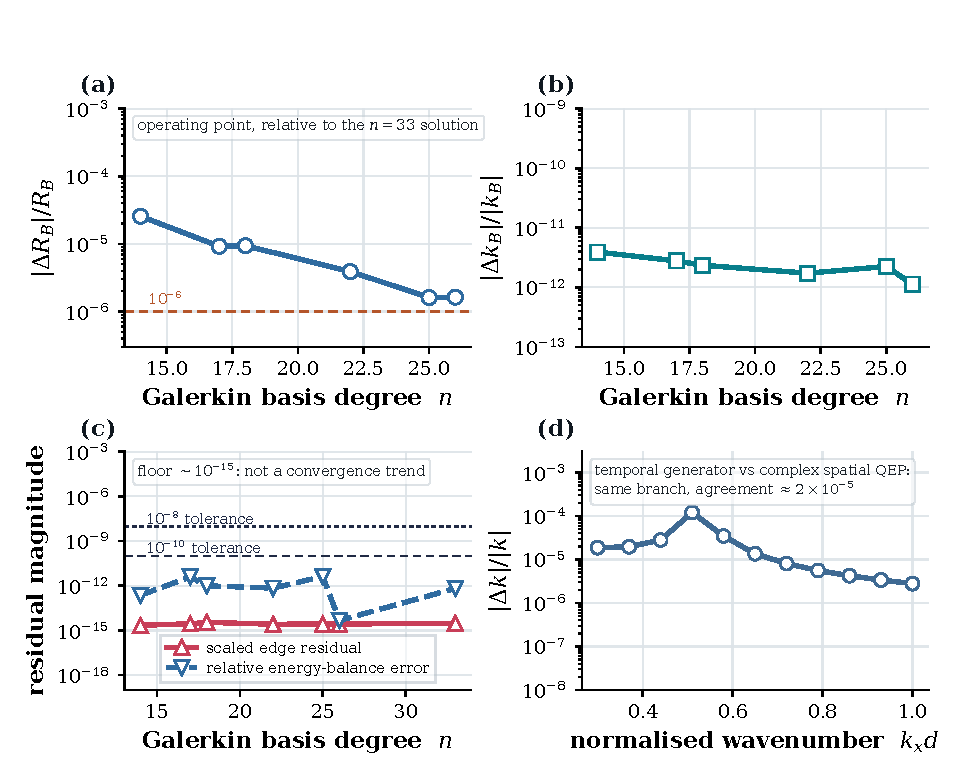
\includegraphics[width=0.95\textwidth]{figures/fig09_validation.pdf}
\caption{Convergence and consistency checks at the operating point. (a) Error of $R_B$ and (b) of the backward wavenumber against the Galerkin degree, relative to the $n=33$ solution; (c) edge residual and energy-balance error; (d) temporal-generator against spatial eigenvalue routes.}
\label{fig:fig09}
\end{figure}


\Cref{fig:fig10} shows the solved field.  Panels (a) and
(b) show the incident and backward intensities on a shared logarithmic color
scale over $x\in[-60,1.5]\,\si{\micro\metre}$ and
$y\in[-45,45]\,\si{\micro\metre}$; the vertical line at $x=0$ is the edge, the
plate lies to its left, and the intensities are normalized to a common maximum
so that the backward field is visibly weaker by one to three decades.  The
incident field approaches the edge at $+10.0^{\circ}$ and the backward field
leaves it at $-27.9^{\circ}$, both measured from the thickness-integrated
Poynting flux and from the $x$ axis along the propagation direction (the $+x$ direction for the incident field, the $-x$ direction for the backward field), positive towards $+y$.

Panel (c) is a schematic, but its arrows are not drawn by hand: they are the
solved directions.  The two wavenumbers point into the plate,
$\vect{k}_i\propto(1,0.176)$ and $\vect{k}_B\propto(1,0.529)$, because $k_y$ is
positive and both axial wavenumbers are real and positive.  The incident flux
follows its wavenumber, $\vect{P}_i\propto(1,0.176)$, whereas the backward flux
is $\vect{P}_B\propto(-1,-0.529)$: the backward mode carries energy in $-x$ and
in $-y$ simultaneously, so its energy transport is opposite in both components
to its own phase direction, and the two flux arrows are the geometric content of
the word ``negative''.  Panel (d) shows the two components of
the backward flux against $k_yd$; both are negative throughout the box, and both
tend to a common small value as $k_yd\to0.2$.

\begin{figure}[htbp]
\centering
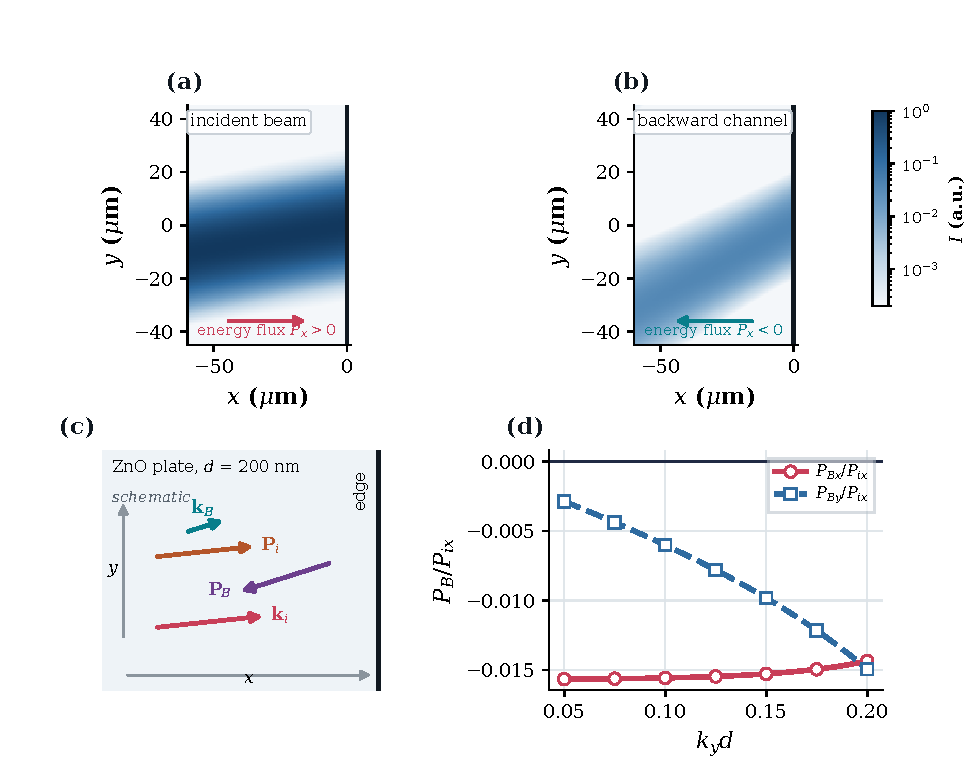
\includegraphics[width=0.95\textwidth]{figures/fig10_field.pdf}
\caption{Field maps and flux directions at the operating point. (a) Incident and (b) backward intensity (arbitrary units, common logarithmic scale) for a Gaussian superposition in $k_yd$ of standard deviation $0.022$ about $0.1298$, edge at $x=0$; (c) schematic of wavenumber and flux directions; (d) components of the backward flux against $k_yd$.}
\label{fig:fig10}
\end{figure}

\subsection{Carrier density and structural loss at the fold}
\label{sec:results_sens}

The two sweeps above vary the carrier density over a factor of three and contain no
loss other than carrier conduction and diffusion.  Because the conversion is largest where the incident
flux nearly vanishes, both limits were tested with the same branch-following definition of $R_B$
($L=10\,d$, $k_yd=0.1298$, $H=0$).

The search for the fold was repeated at six densities from
$2\times10^{18}$ to $2\times10^{23}\,\si{\per\cubic\metre}$, which takes $Q=d/L_D$ from $0.075$ to $24$.  This range covers the densities of nominally undoped ZnO compiled in Table~VII of \cite{ozgur2005zno}, $8\times10^{19}$--$5\times10^{23}\,\si{\per\cubic\metre}$, up to its upper end.  The
maximum falls from $0.943$ through $0.828$ to $0.545$ over the first three densities ($2\times10^{18}$, $2\times10^{19}$, $2\times10^{20}\,\si{\per\cubic\metre}$), with the argmax inside the raster.  From
$2\times10^{21}\,\si{\per\cubic\metre}$ upward the largest sampled value in a window of $\pm0.03$ about the
fold lies on the edge of the window, so the entries ($\ge0.168$, $\ge0.043$ and $\ge0.174$) are lower bounds and the maximum itself was not located.  At the operating
point, which was swept over a wider range than the fold search, the share stays between $0.0158$ and $0.0410$ over the whole range $2\times10^{18}$ to
$6\times10^{23}\,\si{\per\cubic\metre}$, and its linewidth peaks near $2\times10^{22}\,\si{\per\cubic\metre}$ at
\SI{8.7}{\mega\hertz}.  The statement of \cref{sec:results_material} that the density sets the loss but not the
partition therefore holds for the range of \cref{fig:fig02}; at the fold the partition depends on the density through the loss.


For orientation, Zhang et al.\ \cite{zhang2025pscplate} find for a simply supported plate under static load and in free vibration that the semiconductor coupling is active only within a window of initial electron concentration, which moves to larger concentrations as the plate becomes thinner; the concentration at which their damping is largest is $10^{18.6}$, $10^{19.6}$ and $10^{20.6}\,\si{\per\cubic\metre}$ for $h=30$, $3$ and $0.3\,\si{\micro\metre}$.  The present plate ($d=\SI{200}{\nano\metre}$, $n_0\le3\times10^{18}\,\si{\per\cubic\metre}$ in the main sweeps) lies below these values, so the carrier results describe the weakly conducting side of that window.  For shear-horizontal waves in ZnO plates, Li et al.\ \cite{li2023sh} report that an initial density below $2\times10^{18}\,\si{\per\cubic\metre}$ barely changes the cut-off frequencies and that above $10^{23}\,\si{\per\cubic\metre}$ the plate responds as an elastic one, which is consistent with the density range scanned here.  Dispersion and damping of Rayleigh-type waves in a piezo-thermo-electric semiconductor with fractional and nonlocal effects have also been computed \cite{aldandani2026kg}.


The model contains no intrinsic elastic loss.  To measure the effect of one, the elastic
and gradient-elastic tensors were multiplied by $1-\mathrm i\eta$ (time dependence $e^{-\mathrm i\omega t}$), a loss tangent $\eta$, i.e.\ a
quality factor $1/\eta$, with the carrier terms unchanged.  The form and the values of $\eta$ are assumed; none is taken from a measurement.  Viscoelastic loss of the Kelvin--Voigt type has been treated for nonlocal piezo-semiconductors elsewhere \cite{gupta2026heatmap}.
The frequency was scanned over 41 values within $\pm3\times10^{-3}$ of the lossless fold frequency and the largest $R_B$ is
reported, so that each entry is a lower bound on the maximum over frequency.  Refining the scan around its largest value in four successive steps, down to a window of $7.5\times10^{-7}$ in relative frequency, changes the entries to $0.6003$ and $0.1967$, so the figures quoted below are converged in frequency.  The scan shows that $\eta=10^{-5}$
lowers the maximum from $0.943$ to $0.600$ and $\eta=10^{-4}$ to $0.197$, while
$|\Imag k_{ix}|d$ rises from $1.0\times10^{-3}$ to $8.1\times10^{-3}$ and $2.0\times10^{-2}$.  This is the square-root response of the
spatial roots to a small loss near a zero-group-velocity point.  For $\eta\ge10^{-3}$ the port selection finds no
propagating incident mode in the scan window and the entries are not evaluated.  The value
$0.943$ is therefore that of a plate whose only loss is carrier conduction, and it should be read as an upper bound
for a real plate.


\section{Conclusions}
\label{sec:conclusions}

In this work we have computed the scattering of a guided mode at the free edge of
an n-type ZnO plate ($6mm$ symmetry) described by strain-gradient elasticity,
piezoelectricity, flexoelectricity and linearized electron drift--diffusion, with
one added carrier--strain-gradient enthalpy and its reciprocal partners.  The main
findings are as follows.

\begin{enumerate}
\item At $k_xd=0.736$ ($f=\SI{16.68}{\giga\hertz}$) the backward branch carries
\SI{1.93}{\percent} of the incident power.  Along the same branch the share rises
to \SI{94.29}{\percent} at $k_xd=0.52719$ ($f=\SI{16.6547}{\giga\hertz}$), where the
group velocity vanishes and the backward wavenumber approaches the incident one to
within \SI{0.4}{\percent}.  The response has a single peak, and its maximum is a local maximum within the window examined, and the value changes by less than $10^{-5}$
between Galerkin degrees 14 and 34.
\item These numbers are modal shares and not reflectances.  The propagating
outgoing modes carry \SI{99.98}{\percent} of the incident power at the operating
point and \SI{100.05}{\percent} at the maximum, that is, all of it to within
\SI{0.1}{\percent}; the excess over unity is of the order of the interference term, $+5.2\times10^{-4}$ at the reference plane.  At the maximum the incident flux itself has fallen by a factor
$131$ because the branch lies at a zero-group-velocity fold, so a maximal share occurs together with a minimal transported power.
\item The conversion is a property of the backward branch and not of the added
coupling.  With $H=0$ the shares at both points are those of the plate without the
coupling.  The classical plate ($\ell=0$) has a backward interval of its own, with
its fold at $k_xd=0.824$ ($f=\SI{13.69}{\giga\hertz}$); the gradient length
$\ell/d=0.25$ moves the fold to $k_xd=0.527$ and $\SI{16.65}{\giga\hertz}$.  At the
control frequencies of \cref{tab:controls}, which lie on a different classical branch, the classical plate has no backward member, the specular
reflection being its only negative-power outgoing mode.
\item The carrier coupling acts through conduction loss.  At
$|H|=0.05H^{*}$ it reduces the partition by \SI{1.21}{\percent} at the operating
point and by \SI{36.1}{\percent} at the maximum, of which 22.3 percentage points are
propagation loss between the edge and the reference plane.  When the maximum is
searched again at each coupling level it shifts and its upper bound falls, so the
coupling lowers the achievable conversion as well as displacing it.
\item The energy balance closes: the flux at the reference plane equals the edge
flux plus the conduction loss to better than $10^{-11}$ of the incident power, with
the interference term reported separately and no evanescent mode counted as
transported power.
\item At the fold the share is sensitive to loss.  It falls from $0.943$ to $0.545$ when the carrier density rises from $2\times10^{18}$ to $2\times10^{20}\,\si{\per\cubic\metre}$, and to $0.600$ and $0.197$ when a loss tangent of $10^{-5}$ and $10^{-4}$ is added to the elastic constants (\cref{sec:results_sens}); the model contains no other elastic loss, so $0.943$ is an upper bound for a plate with intrinsic damping.
\end{enumerate}

Several limitations should be kept in view.  The gradient length, the
flexoelectric coefficient and the coupling tensor are assumed values, the
carriers are linearized about a uniform doping, and the plate has a single edge.
The corner line force is small but finite in the computed field: it is
$8.4\times10^{-2}$ of the incident corner scale at the operating point and
$3.3\times10^{-3}$ at the maximum.  It decays as a power of the Galerkin degree, with the same exponent in three independent configurations, and the partition moves by
$3.9\times10^{-6}$ over the same range; the closure is therefore shown as a bound, with the decay exponent taken from the computed values.  The added
term has the structure of the chemo-mechanical coupling given in \cite{qu2025thermodynamic}, which that article neglects in its main text; the
comparison with its free-energy decomposition was made through \cite{hu2025computational} and checked against the article itself.  What the present analysis supplies is the modal partition of a slow guided branch
near its zero-group-velocity point, resolved mode by mode rather than in total power.



\section*{Data availability}
All data generated or analysed in this study are included in this article; further numerical detail is available from the corresponding author on reasonable request.

\section*{Declaration of generative AI and AI-assisted technologies in the manuscript preparation process}
During the preparation of this work the author used Claude (Anthropic) to check
equations and numerical results, to verify
bibliographic records and to edit the language. After using this tool, the author
reviewed and edited the content as needed and takes full responsibility for the
content of the publication.

\appendix
\section{Detailed mathematical derivations}
\label{app:derivations}

This appendix contains the calculations that are used in the article but whose
length would interrupt it: the element matrices of the Legendre basis, five
worked matrix elements, the construction of the blocks \eqref{eq:block} from the
weak equations, the edge-matching system, the normalization of the modal power,
and one end-to-end numerical evaluation of the reported share.

\subsection{Element matrices of the Legendre basis}

Three coordinates appear in the formulation and they must be separated before
any integral is written, because the orthonormality of the basis and the size of
the element matrices both depend on which one is meant.  The physical coordinate
is $z\in[-d/2,d/2]$.  The non-dimensional coordinate of the field equations is
$\zeta=2z/d\in[-1,1]$, with $\dd z=(d/2)\dd\zeta$.  The basis is generated on a
third, the half-interval variable
\begin{equation}
\label{eq:app_measures}
s=\frac{z}{d}=\frac{\zeta}{2}\in\Bigl[-\tfrac12,\tfrac12\Bigr],
\qquad
\dd s=\frac{\dd z}{d}=\frac{\dd\zeta}{2},
\end{equation}
and each element matrix in this appendix is an integral over $s$ with the
measure $\dd s$.  The basis is
\begin{equation}
\label{eq:app_basis}
b_j(s)=\sqrt{2j+1}\,P_j(2s),\qquad j=0,\dots,N-1,
\end{equation}
with $N$ the number of basis functions per field.  Since
$\int_{-1}^{1}P_iP_j\dd\zeta=2\delta_{ij}/(2j+1)$, the Gram matrix in the $s$
measure is
\begin{equation}
\label{eq:app_mass}
\int_{-1/2}^{1/2}b_ib_j\,\dd s
=\frac{2j+1}{2}\int_{-1}^{1}P_iP_j\,\dd\zeta=\delta_{ij},
\end{equation}
the first factor being the Jacobian of $s=\zeta/2$ and the second the Legendre
normalization.  The same integral in the $\zeta$ measure is
$\int_{-1}^{1}b_ib_j\dd\zeta=2\delta_{ij}$: the two differ by just the Jacobian, and the mass matrix that multiplies $\dot{\vect q}$ in the weak form is
the identity only in the $s$ measure.  Hence all statements below are made with $\dd s$, and the derivative in $S_{ij}$ is $\dd_s=\dd/\dd s$; in the $\zeta$
coordinate $\dd_s=2\dd/\dd\zeta$, which is the factor of two that appears in all strain-gradient entries.

The stiffness matrix is $S_{ij}=\int b_i'b_j'\dd s$.  For $i=j$ the chain rule
gives $b_j'(s)=2\sqrt{2j+1}\,P_j'(2s)$, so
\begin{equation}
\label{eq:app_S}
S_{jj}=4(2j+1)\int_{-1/2}^{1/2}\bigl(P_j'(2s)\bigr)^{2}\dd s
=2(2j+1)\,j(j+1),
\end{equation}
where $\int_{-1}^{1}(P_j')^{2}\dd\zeta=j(j+1)$ is the classical companion of the
Legendre equation and the factor $2$ collects $4\times\tfrac12$.  The weighted
form of that identity is the one that follows directly from the equation, and it is derived here because this step is usually skipped.  Multiplying
$\bigl[(1-\zeta^{2})P_j'\bigr]'=-j(j+1)P_j$ by $P_k$ and integrating by parts, the
boundary term carrying the factor $(1-\zeta^{2})$ vanishes at both ends and
\begin{equation}
\label{eq:app_S_weighted}
\int_{-1}^{1}(1-\zeta^{2})P_j'P_k'\,\dd\zeta
=\frac{2j(j+1)}{2j+1}\,\delta_{jk},
\end{equation}
which is the orthogonality of the derivatives under the weight
$(1-\zeta^{2})$; \eqref{eq:app_S} is its unweighted companion and is used here
only through the closed form it implies.  The discrete matrix checks both, and so
does an independent quadrature rule of a different order
(\cref{app:repro}): the assembled $S_{jj}$ equals $2j(j+1)(2j+1)$ for every
$j\le N-1$ at all degrees used in this article, to $2\times10^{-11}$ or better
in absolute value.

For $i\neq j$ the parity of $P_i'P_j'$ leaves $S_{ij}\neq0$ only when $i$ and $j$
have the same parity, and
\begin{equation}
\label{eq:app_S_off}
S_{ij}=2\sqrt{(2i+1)(2j+1)}\int_{-1}^{1}P_i'P_j'\,\dd\zeta ,
\end{equation}
which explains the structure of \eqref{eq:app_S_matrix}: the matrix is
real and symmetric and it vanishes between basis functions of opposite parity,
but the same-parity entries are not confined to a band.  At $N=6$ the entry
$S_{15}=22.978$ couples indices four apart, and at any $N$ the row $i$ has
non-zero entries in each column $j\le i$ of the same parity, so the matrix is
not tridiagonal and has no fixed bandwidth; what bounds it is the parity rule,
not a band.  At $N=6$ the matrix is
\begin{equation}
\label{eq:app_S_matrix}
\mathsf S=
\begin{pmatrix}
0&0&0&0&0&0\\
0&12&0&18.330&0&22.978\\
0&0&60&0&80.498&0\\
0&18.330&0&168&0&210.60\\
0&0&80.498&0&360&0\\
0&22.978&0&210.60&0&660
\end{pmatrix},
\end{equation}
whose diagonal is \eqref{eq:app_S} entry by entry.  Equation
\eqref{eq:app_S_matrix} is the entire gradient-energy content of the
discretization for a single field: it is real, symmetric and independent of the
material, and each strain-gradient block of \eqref{eq:block} is this matrix
multiplied by an elastic modulus and by $\lambda^{2}$.

Two further element matrices are needed.  The potential space of the grounded
problem is spanned by
\begin{equation}
\label{eq:app_pot}
\psi_j(s)=b_j(s)-r_j\,b_{j+2}(s),\qquad
r_j=\sqrt{\frac{2j+1}{2j+5}},\qquad j=0,\dots,N_\varphi-1 ,
\end{equation}
which vanishes at $s=\pm\tfrac12$ for every $j$ because $P_j(\pm1)=(\pm1)^j$ and
$r_j$ is exactly the ratio that makes the two terms cancel; $N_\varphi=N-2$,
since $\psi_j$ needs $b_{j+2}$ up to $j=N_\varphi-1$, i.e.\ $b_{N-1}$.  The two
matrices that couple the charge are then distinguished by which index is the test
index.  Testing Gauss's law with $\psi_i$ against the carrier basis $b_j$ gives
\begin{equation}
\label{eq:app_charge}
\bigl(\mathsf C\bigr)_{ij}\equiv\int_{-1/2}^{1/2}\psi_i\,b_j\,\dd s
=\delta_{ij}-r_i\,\delta_{j,i+2},
\qquad i=0,\dots,N_\varphi-1,\quad j=0,\dots,N-1 ,
\end{equation}
that is a unit matrix minus one band above the diagonal, with the coefficient
$r_i$ carrying the \emph{row} index.  The reciprocal matrix that appears in the
carrier equation is its transpose,
\begin{equation}
\label{eq:app_charge_T}
\bigl(\mathsf C^{\mathsf T}\bigr)_{ij}\equiv\int_{-1/2}^{1/2}b_i\,\psi_j\,\dd s
=\delta_{ij}-r_j\,\delta_{i,j+2},
\end{equation}
which has the band below the diagonal and the coefficient $r_j$ on the column
index.  Both appear in \eqref{eq:block}: $-\mathsf C$ in the potential row and
$-\mathsf C^{\mathsf T}$ in the carrier row, entering through the single term
$-\int W_i^{*}W_j$ whose test and trial functions share the potentials.  Writing
$r_j$ where $r_i$ belongs, or transposing the two, gives a matrix that differs
from the assembled one by $0.2981$ in the largest entry at degree four, so the orientation is stated here and not left to the reader.  Finally
the dielectric matrix is
$\kappa_{33}\int\psi_i'\psi_j'\dd s+\kappa_{11}k_y^{2}\int\psi_i\psi_j\dd s$,
with
\begin{equation}
\label{eq:app_diel}
\int_{-1/2}^{1/2}\psi_i'\psi_j'\,\dd s
=S_{ij}-r_jS_{i,j+2}-r_iS_{i+2,j}+r_ir_jS_{i+2,j+2},
\end{equation}
in which the second and third terms are equal because $\mathsf S$ is symmetric,
and the first term is not $S_{ij}$ alone: the grounded basis removes a band of
the stiffness exactly as it removes a band of the mass.

\subsection{Five worked matrix elements}

The entries below are evaluated at the operating point $k_xd=0.7362$,
$k_yd=0.1298$, $\omega=7.6334\,c_s/d$ and at polynomial degree $p=4$, i.e.\
$N=p+1=5$ basis functions per field, $n_{\mathrm{u}}=3N=15$, $n_\varphi=N-2=3$,
$n_\mu=N=5$ and $n_{\mathrm{w}}=5p+3=23$ unknowns.  That is the smallest degree at
which the parity structure and the grounded bands are both visible; the reported
results use $p=22$, with $p=18$ to $34$ examined, where the same formulas hold with larger matrices.
All entries are in the scaled units of the solver: stresses divided by
$c_{44}$, electric displacement by $\sqrt{c_{44}\kappa_{33}}$ and electric field by $\sqrt{c_{44}/\kappa_{33}}$, permittivities by
$\kappa_{33}$, so the numbers are dimensionless.

\begin{enumerate}
\item \emph{Compressibility (mass) entry}, carrier row and column:
\begin{equation}
\label{eq:app_w1}
-\int_{-1/2}^{1/2}b_ib_j\,\dd s=-\delta_{ij}
\qquad\text{so that}\qquad
\bigl(\mathsf A_{00}\bigr)_{\mu_0\mu_0}=-1 ,
\end{equation}
reproduced as $-1$ to $7\times10^{-15}$.
\item \emph{Transport entry.}  The carrier gradient enters the weak form without a
power of $k_x$ through its transverse part and with one power through its axial
part, so the $k_x^{0}$ block holds the transverse wavenumber and the $k_x^{2}$
block the axial one:
\begin{equation}
\label{eq:app_w2}
\bigl(\mathsf A_{00}\bigr)_{\mu_i\mu_j}\Big|_{\text{transport}}
=-\frac{\ii\alpha_{\mathrm d}}{\omega}\Bigl[k_y^{2}\,\delta_{ij}+S_{ij}\Bigr],
\qquad
\bigl(\mathsf A_{11}\bigr)_{\mu_i\mu_j}\Big|_{\text{transport}}
=-\frac{\ii\alpha_{\mathrm d}}{\omega}\,\delta_{ij} ,
\end{equation}
so that the polynomial operator reproduces
$-\ii\alpha_{\mathrm d}\bigl(k_x^{2}+k_y^{2}+S_{ij}\bigr)/\omega$.  With
$\alpha_{\mathrm d}/\omega=0.108509$ and $k_y^{2}=0.016848$ the
diagonal of \eqref{eq:app_w2} is
\begin{equation}
\label{eq:app_w2_values}
-\ii\,1.828\times10^{-3},\quad -\ii\,1.3039,\quad -\ii\,6.5124,\quad
-\ii\,18.2314 \qquad (j=0,\dots,3),
\end{equation}
for $S_{jj}=0,12,60,168$, and the $k_x^{2}$ block is
$-\ii\,0.108509$.  The two pieces together reproduce the assembled coefficient of
the polynomial to $3.6\times10^{-15}$.  The growth with $j$ is the discrete
statement that a higher Legendre mode stores more gradient energy, and hence that diffusion penalizes thickness structure.
\item \emph{Carrier--potential entry.}  With the orientations fixed by
\eqref{eq:app_charge}--\eqref{eq:app_charge_T}, the potential row of
$\mathsf A_{00}$ carries $-\mathsf C$ and the carrier row
$-\mathsf C^{\mathsf T}$:
\begin{equation}
\label{eq:app_w3}
\bigl(\mathsf A_{00}\bigr)_{\varphi_i\mu_j}
=-Q\bigl(\delta_{ij}-r_i\,\delta_{j,i+2}\bigr),
\qquad
\bigl(\mathsf A_{00}\bigr)_{\mu_i\varphi_j}
=\bigl(\mathsf A_{00}\bigr)_{\varphi_j\mu_i},
\end{equation}
so the diagonal is $-Q=-0.074635$ and the band is $+Qr_i$, that is $+0.033378$,
$+0.048860$, $+0.055630$ and $+0.059538$ for $i=0,\dots,3$; the first of these is
$Q/\sqrt{5}$ because $r_0=1/\sqrt{5}$, and the sign is positive because the
band of \eqref{eq:app_charge} is negative and the block has the overall minus
of $-\int W_i^{*}W_j$.  In the carrier row the same numbers appear at
$(i,i-2)$, below the diagonal, with the coefficient $r_{i-2}$ carrying the
\emph{trial} (potential) index; the two matrices are transposes of one another, and
the assembled blocks reproduce \eqref{eq:app_w3} to $9\times10^{-16}$.
\item \emph{Gradient-stiffness entry}, out-of-plane row and column:
\begin{equation}
\label{eq:app_w4}
\lambda^{2}\frac{c_{33}}{c_{44}}\,S_{ij}
=0.0625\times5.1395\times S_{ij}
\;=\;3.85,\ 19.27,\ 53.97,\ 115.64 \quad (j=1,2,3,4),
\end{equation}
growing as $j^{3}$ because $S_{jj}\propto j^{3}$: this is the growth that makes
the discrete operator badly scaled before row equilibration, and $115.64$ at $j=4$ is the largest of these entries at
this degree.
\item \emph{Inertia entry}:
\begin{equation}
\label{eq:app_w5}
-\omega^{2}\delta_{ij}=-58.27\,\delta_{ij}\qquad(\omega=7.6334).
\end{equation}
The ratio of the inertia entry to the $j=1$ gradient entry is
$58.27/3.85=15.1$.  It compares two matrix entries at one fixed frequency and
nothing more: the frequency of a thickness mode is an eigenvalue of the coupled
problem \eqref{eq:quartic}, not the ratio of two entries, and no mode frequency is
inferred from it here.
\end{enumerate}

\subsection{Construction of the blocks from the weak equations}

Each of the nine blocks $\mathsf A_{rs}$ is the sum of the eight bilinear forms
listed in \eqref{eq:block}.  Written out with the operators of
\eqref{eq:sector_blocks} and the integrals of the first subsection of this appendix,
the block is
\begin{equation}
\label{eq:app_block}
\begin{aligned}
\mathsf A_{rs}={}&\underbrace{\bigl\langle\mathsf B_r,\mathsf C\mathsf B_s
\bigr\rangle}_{\text{elastic}}
+\underbrace{\lambda^{2}\bigl\langle\partial_\zeta\mathsf B_r,
\mathsf C\,\partial_\zeta\mathsf B_s\bigr\rangle}_{\text{gradient}}
+\underbrace{\bigl\langle\mathsf G_r,\mathsf e\mathsf B_s\bigr\rangle
+\bigl\langle\mathsf B_r,\mathsf e^{\mathsf T}\mathsf G_s\bigr\rangle}_{\text{piezoelectric}}\\
&-\underbrace{\bigl\langle\mathsf G_r,\boldsymbol\kappa\mathsf G_s\bigr\rangle
}_{\text{dielectric}}
+\underbrace{f\bigl[\bigl\langle\mathsf G_r^{(2)},\partial_\zeta\mathsf B_s^{(2)}
\bigr\rangle+\bigl\langle\partial_\zeta\mathsf B_r^{(2)},\mathsf G_s^{(2)}
\bigr\rangle\bigr]}_{\text{flexoelectric}}
-\underbrace{\frac{\ii\alpha_{\mathrm d}}{\omega}
\bigl\langle\mathsf M\mathsf G_r,\mathsf M\mathsf G_s\bigr\rangle}_{\text{transport}}\\
&-\underbrace{\bigl\langle\mathsf W_r,\mathsf W_s\bigr\rangle}_{\text{carrier}}
-\underbrace{\omega^{2}\bigl\langle\mathsf U_r,\mathsf U\bigr\rangle\delta_{r0}
\delta_{s0}}_{\text{inertia}},
\end{aligned}
\end{equation}
with $\langle\vect a,\vect b\rangle=\int_{-1/2}^{1/2}\vect a^{\mathsf H}\vect b\,
\dd s$ in the measure of \eqref{eq:app_measures}.

The powers of $k_x$ are counted by the block indices $(r,s)$ and by nothing else,
and it is written out here because double counting is the usual error.
The strain of a single mode is split once and for all as
\begin{equation}
\label{eq:app_strain_split}
\varepsilon_{ij}=\varepsilon^{(0)}_{ij}+\ii k_x\,\varepsilon^{(1)}_{ij},
\end{equation}
with both coefficient vectors independent of $k_x$:
\begin{center}
\renewcommand{\arraystretch}{1.1}
\begin{tabular}{@{}lcc@{}}
\toprule
component & $\varepsilon^{(0)}_{ij}$ & $\varepsilon^{(1)}_{ij}$ \\
\midrule
$\varepsilon_{xx}$ & $0$ & $b_j$ in the $\widehat u_1$ slot \\
$\varepsilon_{yy}$ & $\ii k_yb_j$ in the $\widehat u_2$ slot & $0$ \\
$\varepsilon_{zz}$ & $b_j'$ in the $\widehat u_3$ slot & $0$ \\
$\varepsilon_{yz}$ & $b_j'$ in $\widehat u_2$, $\ii k_yb_j$ in $\widehat u_3$ & $0$ \\
$\varepsilon_{xz}$ & $b_j'$ in the $\widehat u_1$ slot & $b_j$ in the $\widehat u_3$ slot \\
$\varepsilon_{xy}$ & $\ii k_yb_j$ in the $\widehat u_1$ slot & $b_j$ in the $\widehat u_2$ slot \\
\bottomrule
\end{tabular}
\end{center}
no component contains more than one power of $\ii k_x$, so the split terminates at
first order.  The strain gradient is split the same way, with $\partial_x$ acting
on the test factor and on the trial factor separately, and the block is defined as
the coefficient of $(-\ii k_x)^{r}(\ii k_x)^{s}$ in \eqref{eq:app_block}:
\begin{equation}
\label{eq:app_ar_s}
\mathsf A_{rs}=\bigl\langle\varepsilon^{(r)},\mathsf C\varepsilon^{(s)}\bigr\rangle
+\lambda^{2}\bigl\langle\partial_z\varepsilon^{(r)},\mathsf C\partial_z\varepsilon^{(s)}\bigr\rangle
+\cdots ,
\end{equation}
the remaining terms of \eqref{eq:app_block} being split in the same way.  Two consequences follow in this language.  First, the leading coefficient
is the gradient energy of the axial part of the strain alone,
\begin{equation}
\label{eq:app_A22}
\mathsf A_{22}=\lambda^{2}\bigl\langle\varepsilon^{(1)},\mathsf C\varepsilon^{(1)}\bigr\rangle
\neq0 ,
\end{equation}
which is where the quartic term and the four wave families come from; its rank is $n_{\mathrm u}$ and not $n_{\mathrm w}$, because $\varepsilon^{(1)}$ is
supported on the displacement slots only.  Secondly, no strain component contains
two powers of $\ii k_x$, which is why $\mathsf A_{02}=\mathsf A_{20}=0$ and the polynomial is a quartic in the $(r,s)$ bookkeeping of \eqref{eq:polynomial}, not a sextic: the
$k_x^{4}$ term needs one factor from each side of the gradient energy and cannot
be produced by a single factor carrying two.

The same bookkeeping fixes where the flexoelectric constant can appear.  The only
non-zero component of $f_{ijkl}$ used in this article is $f_{3333}$, which pairs
the field $E_z$ with the gradient component $\eta_{zzz}=\partial_z\varepsilon_{zz}$;
neither contains a power of $k_x$, since $E_z=-\partial_z\varphi$ and
$\varepsilon_{zz}$ is axial, so $f$ enters $\mathsf A_{00}$ and no other block.
That is a statement about the operator, and it explains why a non-zero $f$ can
change the elastic-like term and the double traction without touching the quartic
coefficient $\mathsf A_{22}$: the two constants sit in different blocks, and
neither of them is a $k_x$ power.

\subsection{The edge-matching system}

At the edge $x=0$ the conditions \eqref{eq:bc_edge} are imposed weakly, one row
block per condition and each on the test functions of the field it multiplies.
The normal there is the $x$ direction, not the $z$ direction: the generalized
traction $\bar\sigma_{1j}$ on the $n_{\mathrm u}=3N$ displacement test functions,
the double traction $\tau_{1j1}\equiv\tau_{jxx}$ on the same $n_{\mathrm u}$ test
functions, the normal electric displacement $D_x$ on the $n_\varphi$ potential
test functions and the normal carrier flux $J_x$ on the $n_\mu$ carrier test
functions.  The face quantities $\bar\sigma_{iz}$, $\tau_{izz}$ and $D_z$ of
\eqref{eq:bc_faces_mech}--\eqref{eq:bc_grounded} belong to $z=\pm d/2$; they are
the natural conditions of the expansion in $z$ and are not the edge conditions.
The number of rows is thus
\begin{equation}
\label{eq:app_edge_rows}
m=2n_{\mathrm u}+n_\varphi+n_\mu ,
\end{equation}
with the double-traction block present whenever the hyperstress is non-zero.  At the edge only the axial strain gradient remains:
\begin{equation}
\label{eq:app_edge_tau}
\tau_{ijx}=\ell^{2}c_{ijkl}\eta_{klx} .
\end{equation}
The two gradient couplings of \eqref{eq:tauZnO} act on the normal-derivative
component: $f$ pairs $E_z$ with $\eta_{zzz}$ and $H$ pairs $\Delta n$ with the
same component, so neither appears in \eqref{eq:app_edge_tau}.  The block exists if and only if $\ell\neq0$, independently of $f$ and of $H$: it
is present in cases A, B and D below, and it is empty in the classical limit
$\ell=f=H=0$, where $\tau_{ijx}\equiv0$ and the double-traction statement
degenerates to $0=0$ and does not give a boundary condition.  The case $\ell=0$ with
$f\neq0$ retains a hyperstress but has no axial trace to pair it with, which is
why it is not a case of this model.  Between those cases the edge problem changes
order, and with it the state:

\begin{center}
\renewcommand{\arraystretch}{1.15}
\begin{tabular}{@{}lllccl@{}}
\toprule
case & parameters & $\tau_{ijx}$ & $N_s$ & $m$ & double traction \\
\midrule
A & $\ell\neq0$, $f\neq0$, $H\neq0$ & $\ell^{2}c_{ijkl}\eta_{klx}$ & $2n_{\mathrm w}+2n_{\mathrm u}$ & $2n_{\mathrm u}+n_\varphi+n_\mu$ & required \\
B & $f=0$, $\ell\neq0$ & $\ell^{2}c_{ijkl}\eta_{klx}$ & $2n_{\mathrm w}+2n_{\mathrm u}$ & $2n_{\mathrm u}+n_\varphi+n_\mu$ & required \\
C & $\ell=0$, $f\neq0$ & $0$ (no axial gradient) & $2n_{\mathrm w}$ & $n_{\mathrm u}+n_\varphi+n_\mu$ & \emph{not available} \\
D & $H=0$, $\ell\neq0$ & $\ell^{2}c_{ijkl}\eta_{klx}$ & $2n_{\mathrm w}+2n_{\mathrm u}$ & $2n_{\mathrm u}+n_\varphi+n_\mu$ & required \\
E & $\ell=f=H=0$ & $0$ & $2n_{\mathrm w}$ & $n_{\mathrm u}+n_\varphi+n_\mu$ & absent (identically zero) \\
\bottomrule
\end{tabular}
\end{center}

\noindent Case C is not a case of the present model: the hyperstress would be non-zero while the
second-order state of case E, which has no $\partial_x u$ trace to pair the
double traction with, is the only one available at $\ell=0$.  Thus the formulation admits $\ell=0$ only in the classical limit $f=H=0$, and states that restriction explicitly; it does not assume that $\ell=0$ implies a second-order model.  No
number in this article depends on case C: every reported run has $\ell\neq0$.

With the edge ansatz \eqref{eq:edge_ansatz} and the modal state
$\vect y^{(j)}\in\mathbb{C}^{N_s}$ (the $n_{\mathrm w}$ displacement and
potential coefficients, the $n_{\mathrm u}$ axial traces, and the $n_{\mathrm w}$
and $n_{\mathrm u}$ conjugate rows), the system is
\begin{equation}
\label{eq:app_edge}
\vect y(0)=\vect y_{\text{inc}}+\sum_{j=1}^{M}a_j\,\vect y^{(j)},
\qquad
\mathsf B\vect a=-\vect b_{\text{inc}},
\end{equation}
where the boundary operator acts on a \emph{state} and the boundary matrix on the
modal index,
\begin{equation}
\label{eq:app_edge_R}
\mathsf R=\begin{pmatrix}
\mathsf R_{\Sigma}\\
\mathsf R_{\tau}\\
\mathsf R_{D}\\
\mathsf R_{J}
\end{pmatrix}\in\mathbb{C}^{m\times N_s},
\qquad
\mathsf B=\bigl[\mathsf R\vect y^{(1)}\ \cdots\ \mathsf R\vect y^{(M)}\bigr]
\in\mathbb{C}^{m\times M},
\qquad
\vect b_{\text{inc}}=\mathsf R\,\vect y_{\text{inc}}\in\mathbb{C}^{m},
\end{equation}
so the three objects have three different second dimensions and only the last two
agree.  They do agree, identically, not by accident: the number of
decaying states is half the state dimension, $M=N_s/2=n_{\mathrm w}+n_{\mathrm u}$
in cases A, B and D, and $M=n_{\mathrm w}$ in case E where $N_s=2n_{\mathrm w}$;
with $n_{\mathrm w}=n_{\mathrm u}+n_\varphi+n_\mu$ from \eqref{eq:nw},
\begin{equation}
\label{eq:app_edge_square}
M=n_{\mathrm w}+n_{\mathrm u}=2n_{\mathrm u}+n_\varphi+n_\mu=m
\quad(\ell\neq0),
\qquad
M=n_{\mathrm w}=n_{\mathrm u}+n_\varphi+n_\mu=m
\quad(\ell=0),
\end{equation}
so the edge system is square in all cases and never over- or under-determined.
At degree four ($n_{\mathrm u}=15$, $n_\varphi=3$, $n_\mu=5$, $n_{\mathrm w}=23$)
this is $N_s=76$, $m=M=38$; at degree eighteen ($57$, $17$, $19$, $93$) it is
$N_s=300$, $m=M=150$; at the reported degree twenty-two ($69$, $21$, $23$, $113$)
it is $N_s=364$, $m=M=182$.  The singular-value decomposition is still used, but as a square solve instead of a least-squares fit: the requirement is that the
rank equal the column count at a cut-off of $10^{-12}$ of the largest singular
value, and a deficient system is reported as such and is not regularized.  Row and
column scaling are applied as before, and the conditioning at the operating point
is $1.4\times10^{2}$ after scaling.
\subsection{Normalization of the modal power}

The power \eqref{eq:Px_int} is bilinear in a mode and its conjugate, so the power
carried by the $j$-th outgoing mode scales with the square of its excitation
amplitude and with the normalization of its eigenvector.  The eigenvector is
normalized by $\vect y^{(j)}\to\vect y^{(j)}/\sqrt{\mathsf y^{\mathsf H}\mathsf
M\mathsf y}$, which fixes its mass norm but leaves the \emph{sign} of the power free:
the physical power is
\begin{equation}
\label{eq:app_power}
P_j=|a_j|^{2}\,\mathcal{P}_x\bigl(\vect y^{(j)}\bigr),
\end{equation}
and the degree-invariance of $P_j$ is the test that the normalization has been
applied correctly.  At the operating point, for the backward mode,
\begin{equation}
\label{eq:app_power_numbers}
\begin{aligned}
n=18:&\quad \mathcal{P}_x=-0.0178923,\quad |a|=1.03848,\quad P_B=-0.0192958,\\
n=22:&\quad \mathcal{P}_x=-0.0154248,\quad |a|=1.11846,\quad P_B=-0.0192957,\\
n=26:&\quad \mathcal{P}_x=-0.0132455,\quad |a|=1.20697,\quad P_B=-0.0192957,\\
n=30:&\quad \mathcal{P}_x=-0.0113777,\quad |a|=1.30227,\quad P_B=-0.0192956,
\end{aligned}
\end{equation}
in which the raw power falls by \SI{36}{\percent} and the squared amplitude rises by
\SI{57}{\percent} across the four degrees while the physical power is constant to
the six digits shown.  That constancy is the
numerical statement of \eqref{eq:app_power} and it is why the reported
share is degree-independent at the $10^{-6}$ level of
\cref{tab:refinement}.

\subsection{One end-to-end evaluation of the reported share}

The reported number at the operating point is assembled from five quantities,
each of which is stored with each row of the data: the raw backward power
$\mathcal{P}_x$, the scattering amplitude $|a_B|$, the incident power at the
reference plane, the two attenuation exponents and the reference distance
$L=10\,d$.  The five are quoted below from \emph{one} row, the reported degree
$n=22$, and not mixed with the neighboring degrees of
\eqref{eq:app_power_numbers}, because the raw power and the amplitude both change
with degree even though their product does not:
\begin{equation}
\label{eq:app_RB}
R_B=\frac{|a_B|^{2}\bigl|\mathcal{P}_x\bigr|\,e^{2\Imag k_{Bx}L}}
{P_{\text{inc}}\,e^{2\Imag k_{ix}L}}
=\frac{0.0192957\times0.9998954}{1.0001081}
=\frac{0.0192937}{1.0001081}=0.0192916 ,
\end{equation}
with, at $n=22$,
\begin{equation}
\label{eq:app_RB_inputs}
|a_B|=1.1184598,\quad
|a_B|^{2}=1.250952,\quad
\mathcal{P}_x=-0.015424813,\quad
|a_B|^{2}\bigl|\mathcal{P}_x\bigr|=0.0192957 ,
\end{equation}
the last product being the power the backward port actually carries at the edge.
The factor $e^{2\Imag k_{Bx}L}=0.9998954$ brings it to $x=-L$ with
$\Imag k_{Bx}=-5.2306\times10^{-6}$ per unit $d$, and the incident mode carries
$e^{2\Imag k_{ix}L}=1.0001081$ with $\Imag k_{ix}=+5.4027\times10^{-6}$; both
exponents are degree-independent to the seven digits quoted, so the degree of the
row enters \eqref{eq:app_RB} only through $|a_B|^{2}|\mathcal{P}_x|$.  What the
number measures is the ratio of two physical powers,
$-P_B/P_{\text{inc}}=0.0192916$, and the two exponential factors state at which
plane each power was taken.

The value and its meaning are two different statements and are kept apart.
Equation \eqref{eq:app_RB} evaluates the share at the \emph{operating point},
$1.93$ percent of the incident power at $x=-10\,d$.  The local maximum of the
same quantity over the frequency window, $R_B=0.9428718$, is a property of the
peak row, not of this one, and \eqref{eq:app_RB} neither computes nor implies it.  Reading the operating-point row along the plate, the backward mode carries
$1.93$ percent at $x=-10\,d$ and $1.93\,\%\times e^{-2.13\times10^{-4}}$ at
$x=-20\,d$: the decay of the share is governed by the \emph{difference} of the two
attenuation constants, not by either one of them.

\section{Numerical resolution and convergence}
\label{app:repro}

\paragraph{Resolution.}  The reported solutions use polynomial degree $n=22$, that is
$N=23$ Legendre modes per field ($N-2=21$ for the grounded potential), and every integral is evaluated
with $\max(64,2n+10)$ Gauss--Legendre nodes, which resolves the mass, stiffness
and coupling matrices to machine precision at the degrees used here.  The two
electrical cases differ only in the potential space: the grounded basis is built
from the combinations that vanish on both faces, and the open-circuit basis
keeps all $N$ modes, because a constant potential is not a gauge for a nonzero in-plane wavenumber.  No field is discretized in $x$ or in $y$.

\paragraph{Convergence and conservation.}  Between degree $18$ and degree $30$
both the operating-point share and the branch maximum change by less than
$10^{-5}$, and successive differences at the branch maximum decrease
monotonically with degree.  Refining the quadrature from $64$ to $256$ nodes at
fixed basis changes no reported digit.  The energy identity
\eqref{eq:energy_identity} is satisfied to $4\times10^{-12}$ of the incident
power at the reported solutions, and the partition at the branch maximum varies by $1.0\times10^{-6}$ in absolute terms between
degrees $14$ and $34$.  These are the quantities that
license quoting the shares to the precision used in the text.


\bibliographystyle{unsrt}
\bibliography{references}

\end{document}
